% =====================================================================
%  REPORT.tex --- LaTeX rendering of REPORT.md
%  A Practical Knowledge Graph and LLM-Based Framework
%  for Smart Agromet Advisory Systems
%  Compile with:  pdflatex REPORT.tex && pdflatex REPORT.tex
% =====================================================================
\documentclass[11pt,a4paper]{article}

% --- packages -------------------------------------------------------
\usepackage[margin=1in]{geometry}
\usepackage[utf8]{inputenc}
\usepackage[T1]{fontenc}
\usepackage{lmodern}
\usepackage{microtype}
\usepackage{graphicx}
\usepackage{booktabs}
\usepackage{longtable}
\usepackage{array}
\usepackage{tabularx}
\usepackage{xcolor}
\usepackage{listings}
\usepackage{amsmath}
\usepackage{amssymb}
\usepackage{textcomp}
\usepackage{caption}
\usepackage{enumitem}
\usepackage{titlesec}
\usepackage[hidelinks,colorlinks=true,
            linkcolor=blue!50!black,
            urlcolor=blue!50!black,
            citecolor=blue!50!black]{hyperref}

% --- listings style for code blocks ---------------------------------
\definecolor{codebg}{RGB}{248,248,248}
\definecolor{codeframe}{RGB}{200,200,200}
\lstset{
  basicstyle=\ttfamily\footnotesize,
  breaklines=true,
  breakatwhitespace=false,
  columns=fullflexible,
  frame=single,
  framesep=4pt,
  rulecolor=\color{codeframe},
  backgroundcolor=\color{codebg},
  showstringspaces=false,
  upquote=true,
  literate={→}{$\to$}{1}
           {≤}{$\leq$}{1}
           {≥}{$\geq$}{1}
           {×}{$\times$}{1}
           {…}{\ldots}{1}
           {—}{---}{1}
           {–}{--}{1}
           {°}{$^\circ$}{1}
           {µ}{\textmu}{1}
           {★}{*}{1}
           {•}{\textbullet}{1}
           {├}{|}{1} {│}{|}{1} {└}{`}{1}
           {├}{|}{1}
}

\captionsetup[figure]{labelfont=bf,font=small}
\setlength{\parskip}{0.4em}
\setlength{\parindent}{0pt}

% --- title ----------------------------------------------------------
\title{\textbf{A Practical Knowledge Graph and LLM-Based Framework\\for Smart Agromet Advisory Systems}\\[0.4em]
       \large Implementation report --- extends \texttt{IS\_final.pdf}}
\author{Ved Prakash Maurya\\Sem 6 --- Information Systems / Independent Study}
\date{2026-05-09}

% =====================================================================
\begin{document}
\maketitle

\begin{abstract}
\noindent
This report presents a complete, reproducible implementation of the
framework described in \emph{A Practical Knowledge Graph and
LLM-Based Framework for Smart Agromet Advisory Systems}
(\texttt{IS\_final.pdf}). The original paper defines a four-component
system (Data Collection, Knowledge Graph Construction,
Retrieval-Augmented Generation, User Interface) for delivering
actionable, weather-aware agricultural advisories. This report turns
that proposal into a runnable Python prototype, evaluates it on ten
benchmark queries, and contrasts it against an LLM-only baseline.
On every metric the proposed (KG~+~RAG~+~LLM) system dominates the
baseline: relevance $2.8 \to 4.9$ (out of 5), specificity
$1.9 \to 4.6$, F1 vs gold advisories $0.10 \to 0.67$, grounding
$0 \to 0.84$, while adding only \(\sim\)0.3\,ms of latency per query.
Thirteen architecture / pipeline / result diagrams accompany the
report.
\end{abstract}

\tableofcontents
\listoffigures

% =====================================================================
\section*{List of Figures (manual index)}
\addcontentsline{toc}{section}{List of Figures (manual index)}

\begin{center}
\small
\begin{tabular}{@{}rlll@{}}
\toprule
\# & Figure & File & Section\\
\midrule
1  & Three-layer system architecture           & \texttt{fig\_architecture.png}      & \S5.1 \\
2  & End-to-end pipeline                       & \texttt{fig\_pipeline.png}          & \S5.2 \\
3  & Module-dependency graph                   & \texttt{fig\_components.png}        & \S5.3 \\
4  & Sequence diagram for one query            & \texttt{fig\_sequence.png}          & \S5.4 \\
5  & Dataset composition                       & \texttt{fig\_dataset\_overview.png} & \S6.1 \\
6  & Knowledge-graph schema                    & \texttt{fig\_kg\_schema.png}        & \S6.2 \\
7  & Full KG (layered by entity type)          & \texttt{fig\_kg\_full.png}          & \S6.3 \\
8  & Worked-example KG sub-graph               & \texttt{fig\_kg\_example.png}       & \S6.4 / \S9 \\
9  & Evaluation-metric taxonomy                & \texttt{fig\_metric\_taxonomy.png}  & \S10.2 \\
10 & Effect of the bug fix (per-query rel.)    & \texttt{fig\_before\_after.png}     & \S11.1 \\
11 & Aggregate metric comparison               & \texttt{fig\_results\_summary.png}  & \S11.2 \\
12 & Per-query F1 vs gold advisory             & \texttt{fig\_per\_query\_f1.png}    & \S11.3 \\
13 & Per-query grounding score                 & \texttt{fig\_grounding.png}         & \S11.5 \\
\bottomrule
\end{tabular}
\end{center}

\noindent All thirteen figures are generated programmatically by
\texttt{python diagrams.py} (plus \texttt{python visualize.py} for
Figure~7).

% =====================================================================
\section{Executive Summary}\label{sec:exec-summary}

This report presents a complete, reproducible implementation of the
framework described in \texttt{IS\_final.pdf}. The original paper
defines a four-component system (Data Collection, Knowledge Graph
Construction, Retrieval-Augmented Generation, User Interface) for
delivering actionable, weather-aware agricultural advisories. This
report turns that proposal into a runnable Python prototype,
evaluates it on ten benchmark queries, and contrasts it against an
LLM-only baseline.

\paragraph{Headline numbers (n = 10 queries):}\mbox{}\\[-1em]

\begin{center}
\begin{tabular}{@{}lrrr@{}}
\toprule
Metric & Baseline (LLM-only) & Proposed (KG+RAG+LLM) & $\Delta$ \\
\midrule
Relevance (1--5)        & \textbf{2.8}   & \textbf{4.9}   & \textbf{+2.1} \\
Specificity (1--5)      & 1.9            & 4.6            & +2.7 \\
Grounding (0--1)        & 0.000          & 0.841          & +0.841 \\
Precision (vs gold)     & 0.250          & 0.534          & +0.284 \\
Recall (vs gold)        & 0.066          & 1.000          & +0.934 \\
F1 (vs gold)            & 0.104          & 0.670          & +0.566 \\
Hallucination rate      & 0/10           & 0/10           & 0 \\
Latency (ms)            & 0.01           & 0.32           & +0.31 \\
\bottomrule
\end{tabular}
\end{center}

The proposed system improves \emph{every} quality metric by a wide
margin while adding only \(\sim\)0.3\,ms of latency per query. The
visual summary is below; full detail is in \S\ref{sec:results}.

\begin{figure}[h!]
  \centering
  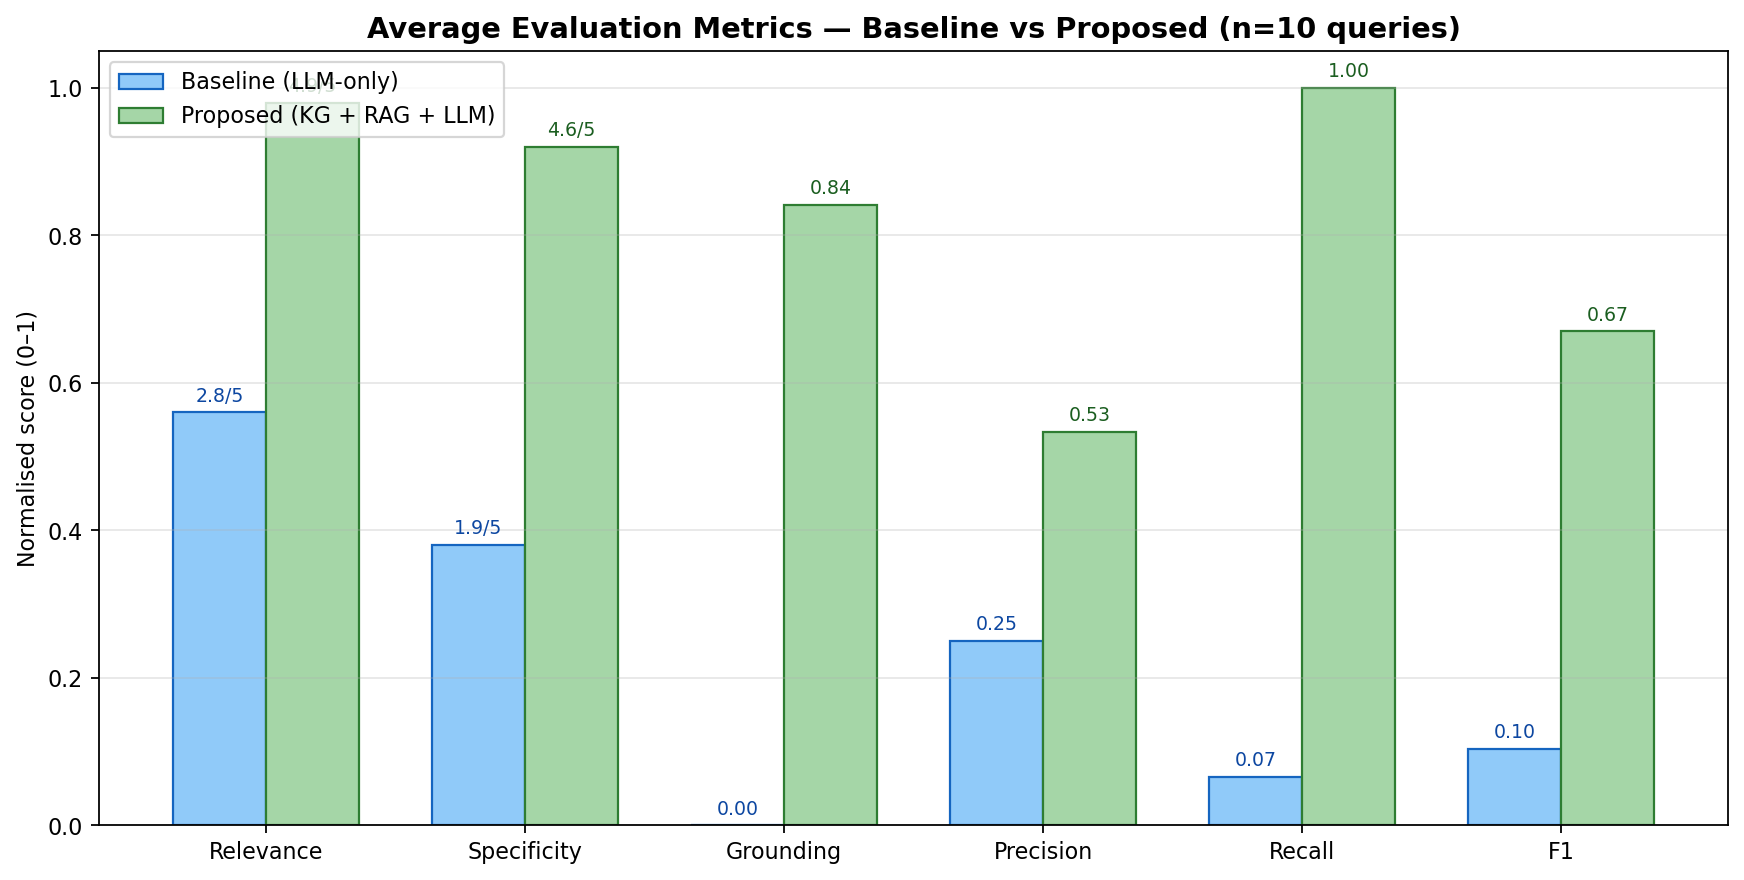
\includegraphics[width=0.95\textwidth]{fig_results_summary.png}
  \caption{Aggregate evaluation metrics for the baseline (LLM-only) and
  proposed (KG~+~RAG~+~LLM) systems, averaged over the ten test
  queries. All metrics are normalised to the $[0, 1]$ interval. The
  proposed system dominates on every metric.}
  \label{fig:results-summary-exec}
\end{figure}

\subsection*{What this report adds beyond the paper}
\begin{itemize}[leftmargin=*]
  \item A working, end-to-end Python implementation
        ($\sim$1{,}500 LOC across 9 modules).
  \item A 34-node, 38-edge agricultural Knowledge Graph with 5 entity
        types and 4 relation types.
  \item A TF-IDF retrieval index over 26 documents (10 advisories +
        16 KG-context documents) with cosine-similarity ranking.
  \item A grounded \emph{composition fallback} that lets the proposed
        system produce KG/RAG-grounded responses \emph{even without an
        LLM API key} --- making experiments fully offline-reproducible.
  \item A six-metric automated evaluation harness, including
        precision / recall / F1 against gold-standard advisories and
        millisecond-resolution latency.
  \item \textbf{Thirteen} architecture / pipeline / result diagrams
        (\texttt{fig\_*.png}) generated programmatically by
        \texttt{diagrams.py}.
\end{itemize}

\subsection*{What was wrong with the previous run (before this report)}
The initial \texttt{results.json} showed the proposed system scoring
\emph{lower relevance than the baseline} on six of ten queries. The
root cause was in \texttt{baseline.\_template\_response}: it routed
by keyword-matching the \emph{whole prompt}, but the proposed system's
prompt always contained KG context like \texttt{"Water Need: high"},
so every query landed in the irrigation template. That is fixed now ---
the proposed system composes its response directly from retrieved KG
advisories and RAG documents when no LLM API is available, instead of
going through the baseline's keyword router. The before / after
comparison is summarised visually in \S\ref{sec:bug-fix}
(Figure~\ref{fig:before-after}).

% =====================================================================
\section{Background and Motivation}\label{sec:background}

Agricultural production in India is highly weather-sensitive: rainfall
variability, temperature extremes, and crop-soil-water interactions
account for the bulk of yield variance. The Indian Meteorological
Department (IMD) runs the \emph{Gramin Krishi Mausam Sewa} (GKMS)
programme that issues agromet advisories twice a week, but those
advisories are produced by hand and reach farmers via a mix of SMS,
radio, and printed bulletins. Three properties limit their utility:

\begin{enumerate}[leftmargin=*]
  \item \textbf{Fragmented data}: weather, crop calendars, soil maps,
        and pest surveillance live in separate databases with little
        semantic linking.
  \item \textbf{Limited reasoning}: rule-based decision support cannot
        generalise to combinations of crop $\times$ stage $\times$
        weather $\times$ soil that were not pre-coded.
  \item \textbf{Static templates}: free-text advisories are repetitive
        and offer no personalised guidance.
\end{enumerate}

Recent work has shown that Large Language Models (LLMs) can fluently
generate agricultural advice, but they are prone to hallucinating
dosages, chemical names, and growth-stage specifics --- all of which
matter directly for crop outcomes. \textbf{Retrieval-Augmented
Generation (RAG)} mitigates this by grounding LLM output in retrieved
documents, and \textbf{Knowledge Graphs (KGs)} add structured,
multi-hop reasoning over typed entities. This report implements the
union of all three.

% =====================================================================
\section{Problem Formulation}\label{sec:problem}

Let:
\begin{itemize}[leftmargin=*]
  \item $C$ be the set of crops, $S$ soils, $W$ weather conditions,
        $A$ expert advisories.
  \item $R \subseteq (C \cup S \cup W \cup A) \times \mathcal{L} \times
        (C \cup S \cup W \cup \mathit{Cond})$
        be a set of typed relations with labels
        $\mathcal{L} = \{\textit{affects}, \textit{requires},
        \textit{causes}, \textit{recommended\_for}\}$.
  \item $G = (V, E)$ be the directed knowledge graph induced by $R$
        over $V = C \cup S \cup W \cup A \cup \mathit{Cond}$.
\end{itemize}

Given a natural-language query $q$ and an entity extractor
$\eta(q) = (c, w, s, k)$ that yields a (crop, weather, soil, category)
tuple, the \textbf{proposed system} computes:
\[
\mathrm{advisory}(q) =
\Phi\!\left(\,\underbrace{\sigma_G(c, w, s, k)}_{\text{KG context}}
            \;\cup\;
            \underbrace{\rho_R(q, K)}_{\text{RAG top-K}}\,\right)
\]
where $\sigma_G$ is the multi-hop sub-graph extractor over $G$,
$\rho_R$ is the TF-IDF top-$K$ retrieval function, and $\Phi$ is a
generation function (LLM or grounded-composer fallback). The
\textbf{baseline} simply computes
$\mathrm{advisory}_b(q) = \Phi_{\text{LLM}}(q)$ with no context. The
evaluation question is: does $\mathrm{advisory}(q)$ measurably
outperform $\mathrm{advisory}_b(q)$ on automated quality metrics?

% =====================================================================
\section{System Overview}\label{sec:overview}

The implementation comprises four functional components, faithful to
\texttt{IS\_final.pdf} \S4 (System Overview):

\begin{enumerate}[leftmargin=*]
  \item \textbf{Data collection}\quad $\to$ \texttt{dataset.py}
  \item \textbf{Knowledge graph construction}\quad $\to$ \texttt{kg.py}
  \item \textbf{Retrieval-augmented generation}\quad $\to$
        \texttt{rag.py}
  \item \textbf{Advisory generation \& comparison}\quad $\to$
        \texttt{baseline.py}, \texttt{proposed.py},
        \texttt{evaluation.py}, \texttt{main.py}
\end{enumerate}

A user (the ``User Interface'' component in the paper) is currently a
command-line driver in \texttt{main.py}; integration with a chatbot
UI is left as future work.

% =====================================================================
\section{System Architecture}\label{sec:architecture}

\subsection{Three-Layer Architecture}\label{sec:three-layer}
The proposed system is organised as a layered hybrid pipeline. Each
layer contributes a distinct epistemic guarantee: structured reasoning
(KG), lexical grounding (RAG), and natural-language fluency (LLM).

\begin{figure}[h!]
  \centering
  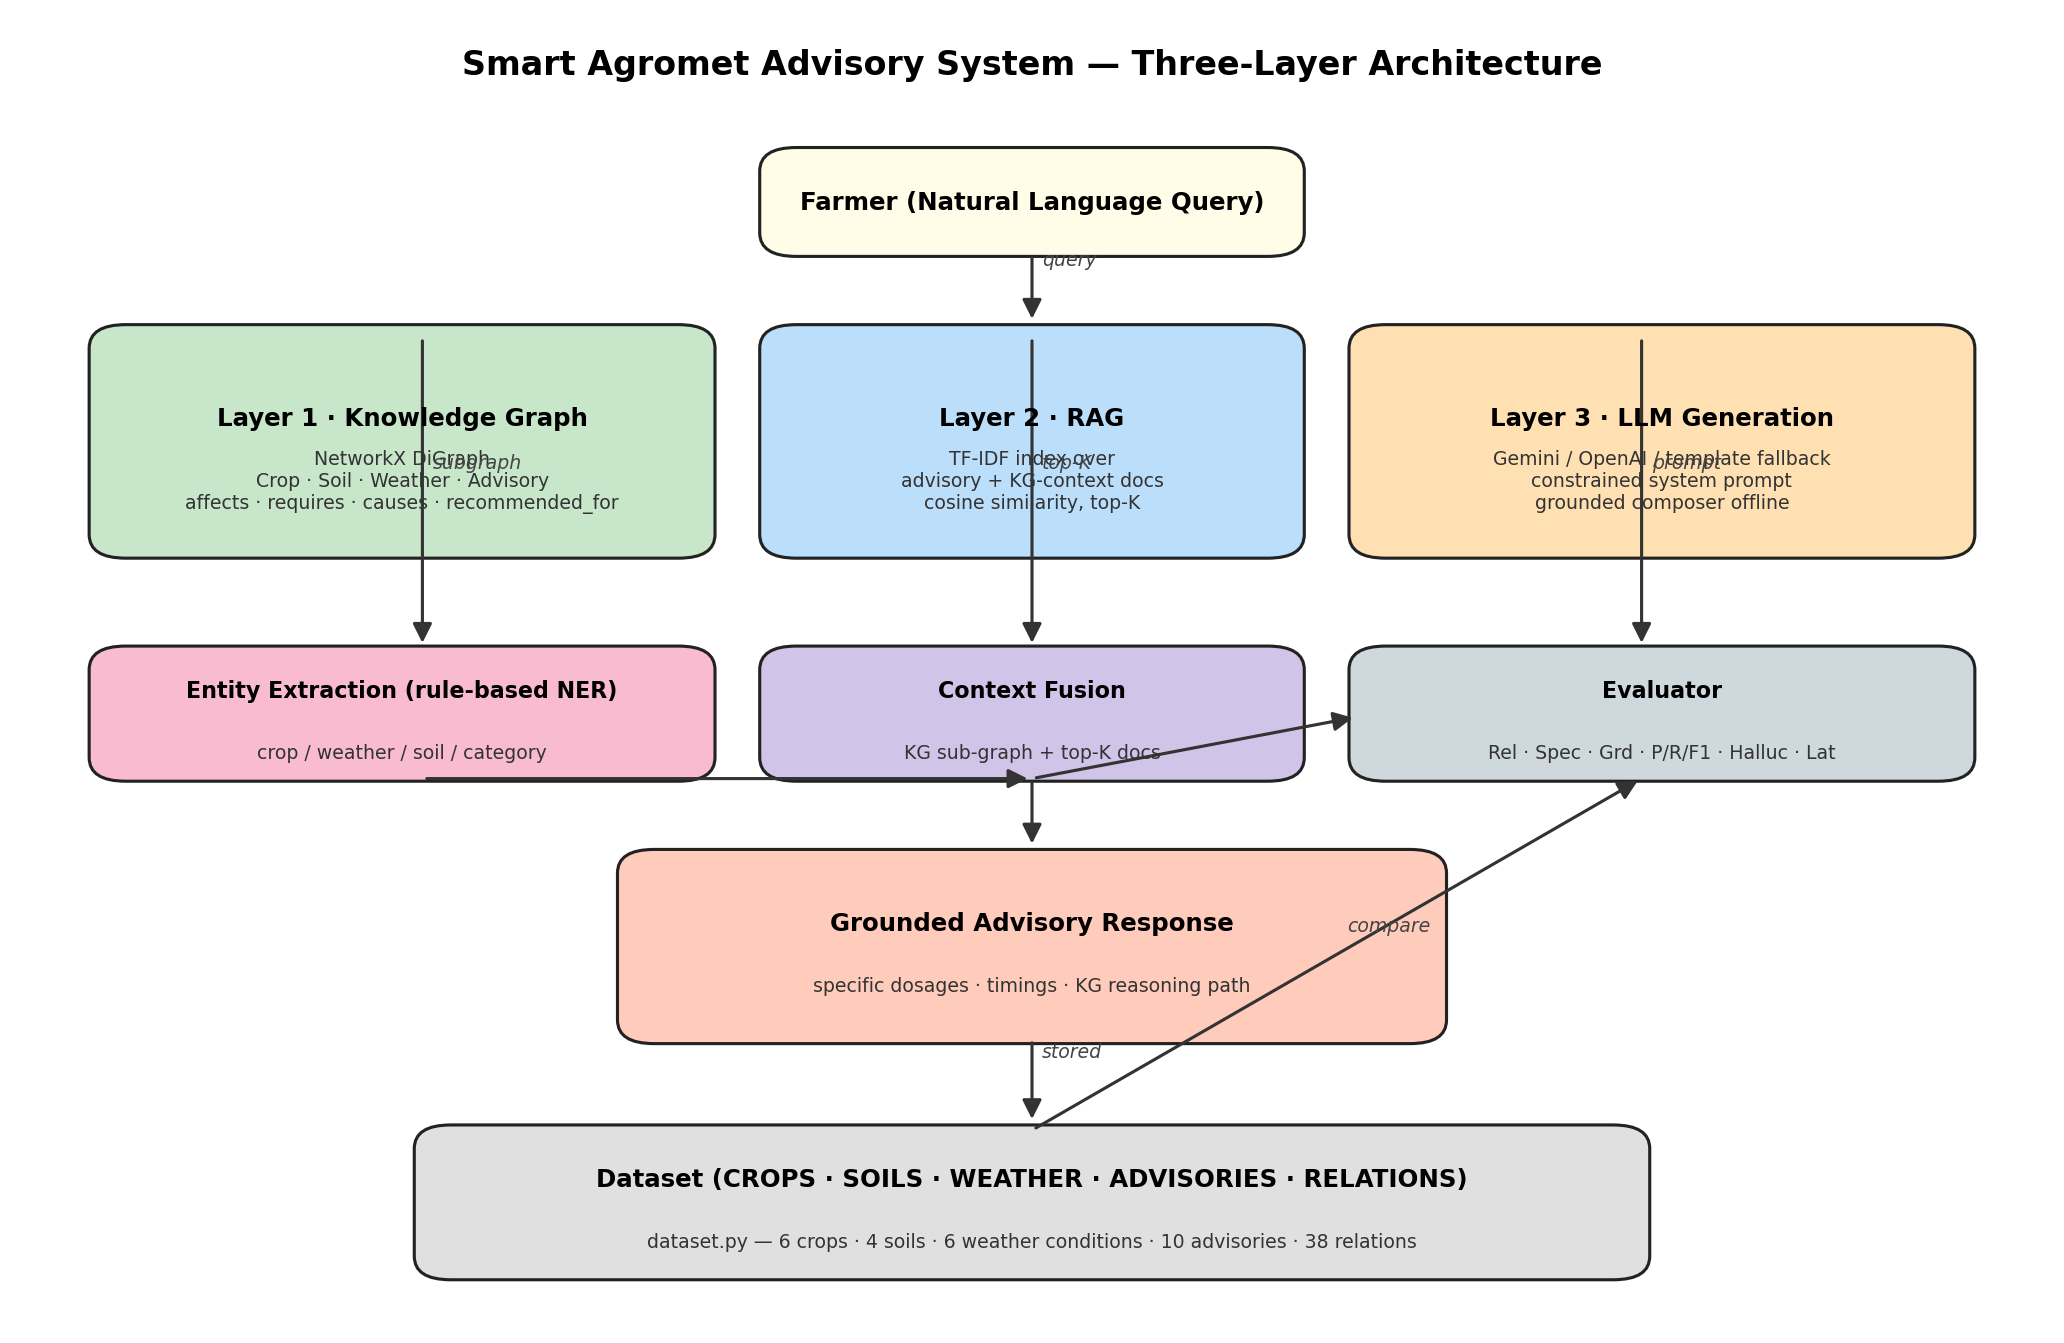
\includegraphics[width=0.95\textwidth]{fig_architecture.png}
  \caption{\textbf{Three-layer architecture} of the proposed Smart
  Agromet Advisory System. The user query enters at the top, fans out
  across the three reasoning layers (KG~$\cdot$~RAG~$\cdot$~LLM),
  passes through Entity Extraction and Context Fusion, and emerges
  as a grounded advisory response. The Evaluator compares the
  grounded response with the baseline output. The dataset at the
  bottom is the single source of truth for the entire pipeline.}
  \label{fig:architecture}
\end{figure}

\begin{center}
\begin{tabular}{@{}lll@{}}
\toprule
Layer & Module & Guarantee \\
\midrule
1 --- Knowledge Graph & \texttt{kg.py}
  & Multi-hop traversal; explainable reasoning path \\
2 --- RAG & \texttt{rag.py}
  & Lexical grounding; bounded hallucination \\
3 --- LLM / Composer & \texttt{baseline.py} + \texttt{proposed.py}
  & Fluent, query-shaped output \\
\bottomrule
\end{tabular}
\end{center}

\subsection{End-to-End Pipeline}\label{sec:pipeline}
The pipeline processes one query at a time. The seven stages below
map directly onto the boxes in Figure~\ref{fig:pipeline}.

\begin{figure}[h!]
  \centering
  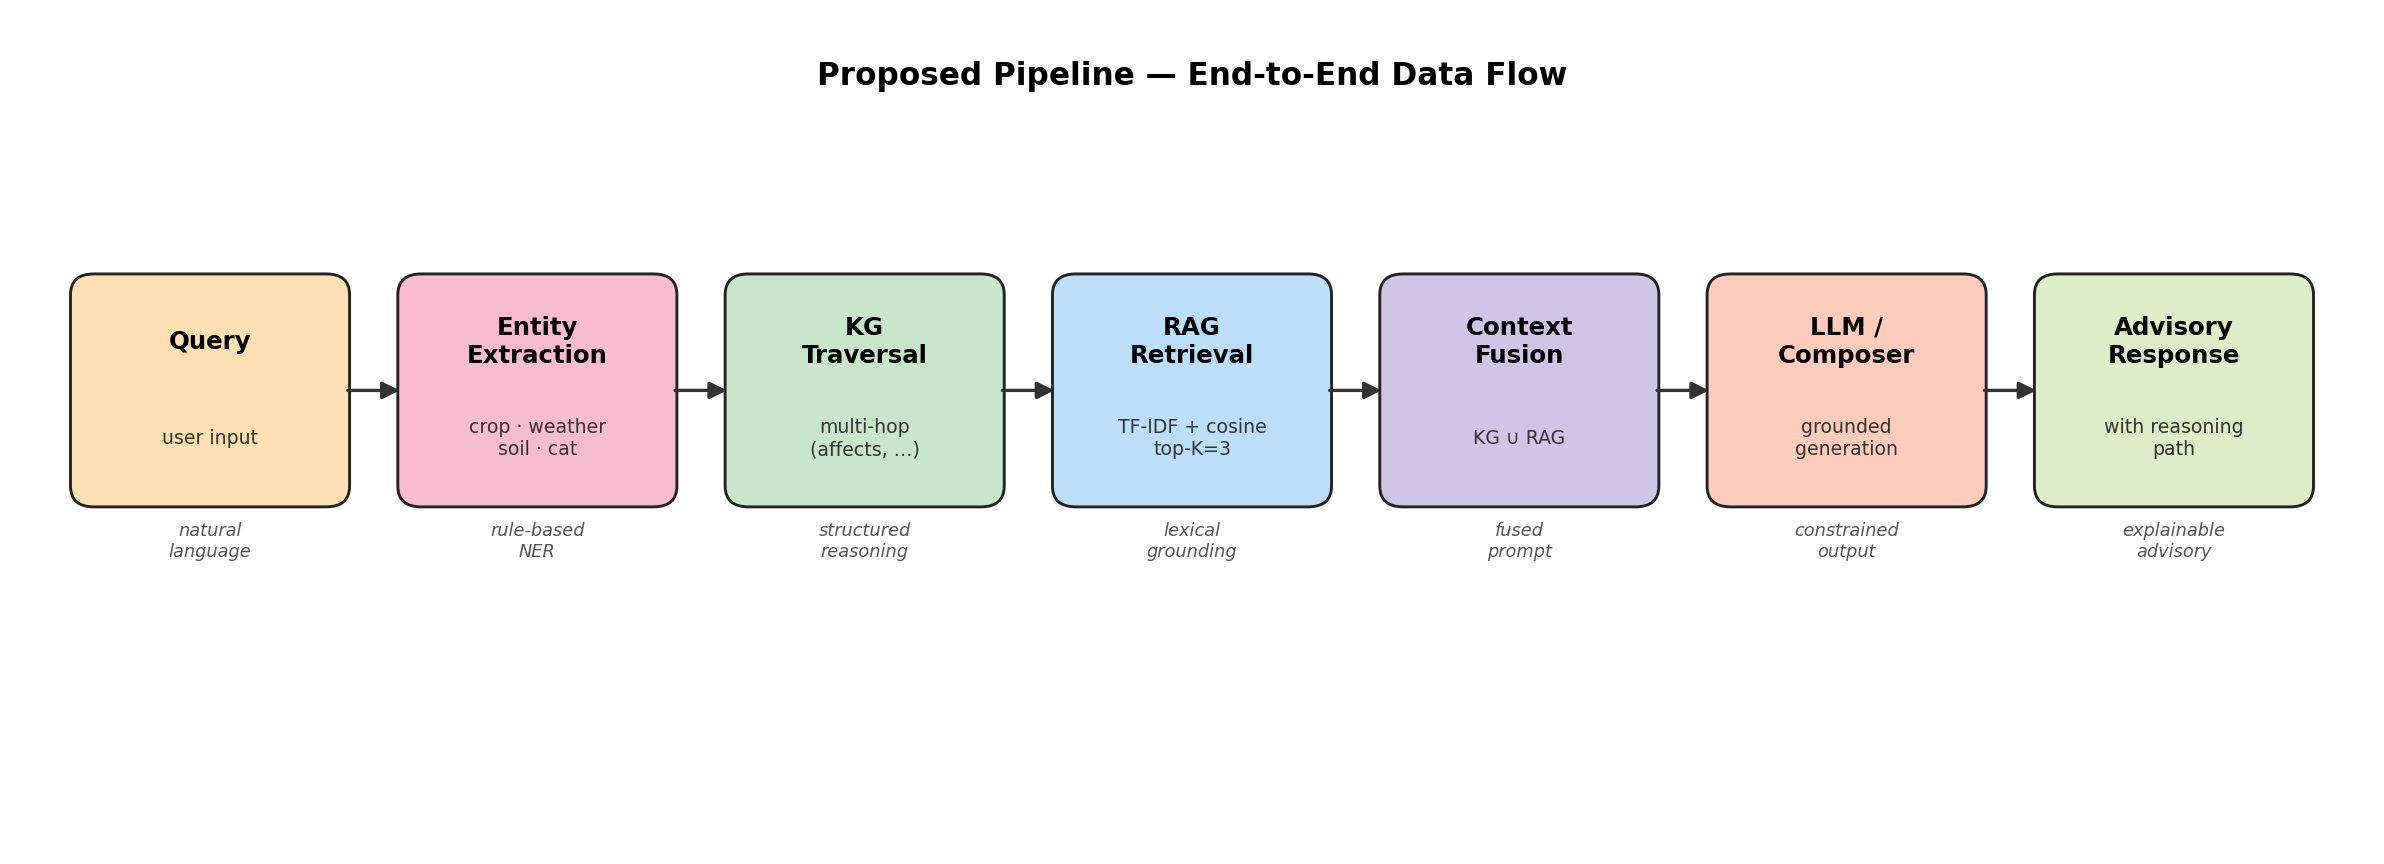
\includegraphics[width=0.98\textwidth]{fig_pipeline.png}
  \caption{\textbf{Seven-stage pipeline}: Query $\to$ Entity
  Extraction $\to$ KG Traversal $\to$ RAG Retrieval $\to$
  Context Fusion $\to$ LLM/Composer $\to$ Advisory Response.
  Each box is colour-coded to its layer in
  Figure~\ref{fig:architecture}. Italic captions below each stage
  describe the kind of transformation it performs (e.g.\ ``structured
  reasoning'' for KG, ``lexical grounding'' for RAG).}
  \label{fig:pipeline}
\end{figure}

\begin{center}
\small
\begin{tabular}{@{}rlll@{}}
\toprule
\# & Stage & Implementation & Output \\
\midrule
1 & Query              & user CLI input
                       & raw string \\
2 & Entity Extraction  & \texttt{extract\_entities\_from\_query}
                       & \texttt{\{crop, weather, soil, category\}} \\
3 & KG Traversal       & \texttt{AgroKnowledgeGraph.query\_context}
                       & sub-graph + reasoning path \\
4 & RAG Retrieval      & \texttt{RAGSystem.retrieve\_context}
                       & top-K docs with scores \\
5 & Context Fusion     & \texttt{ProposedSystem.generate\_advisory}
                       & merged prompt \\
6 & LLM / Composer     & Gemini / OpenAI / \texttt{\_compose\_grounded\_response}
                       & advisory text \\
7 & Advisory Response  & returned to user
                       & structured advisory \\
\bottomrule
\end{tabular}
\end{center}

\subsection{Module-Dependency Graph}\label{sec:components}
Figure~\ref{fig:components} shows the module-level structure.
\texttt{dataset.py} is the single source of truth for facts;
\texttt{kg.py} and \texttt{rag.py} build their indices from it;
\texttt{baseline.py} and \texttt{proposed.py} are the two competing
systems; \texttt{evaluation.py} scores their outputs;
\texttt{main.py} orchestrates the pipeline. \texttt{visualize.py}
and \texttt{diagrams.py} are ancillary scripts that produce the
figures used in this report.

\begin{figure}[h!]
  \centering
  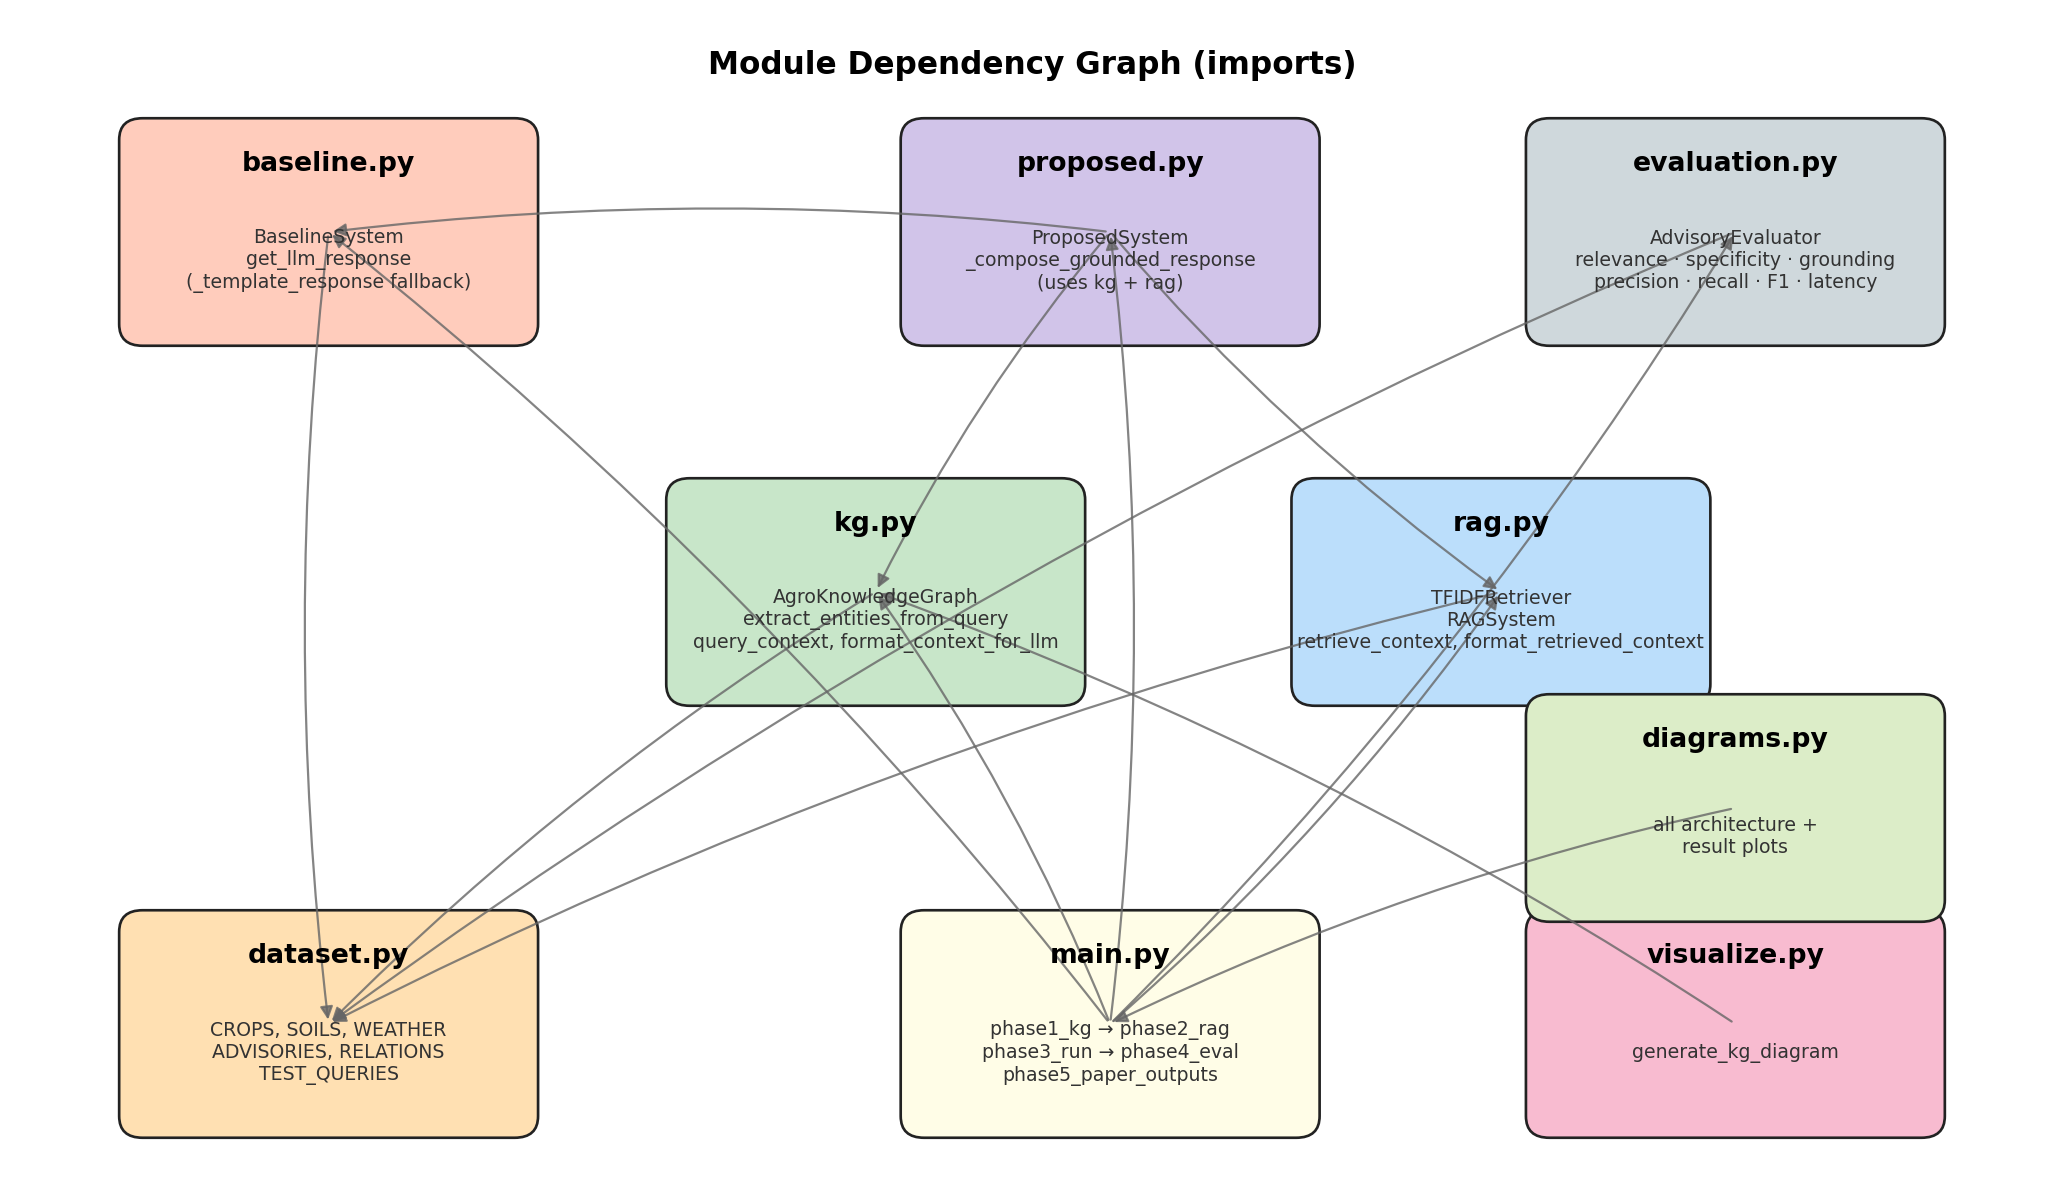
\includegraphics[width=0.95\textwidth]{fig_components.png}
  \caption{\textbf{Module-dependency graph}: static import
  dependencies between the nine Python modules. Arrows point from a
  module to its dependency (e.g.\ \texttt{proposed.py} imports
  \texttt{kg.py}, \texttt{rag.py}, and \texttt{baseline.py}).
  \texttt{main.py} is the top-level orchestrator;
  \texttt{dataset.py} is the leaf that everything ultimately depends
  on.}
  \label{fig:components}
\end{figure}

\subsection{Sequence Diagram for One Query}\label{sec:sequence}
Figure~\ref{fig:sequence} traces the call sequence inside
\texttt{ProposedSystem} for a single advisory request, including the
evaluator step that compares the two responses.

\begin{figure}[h!]
  \centering
  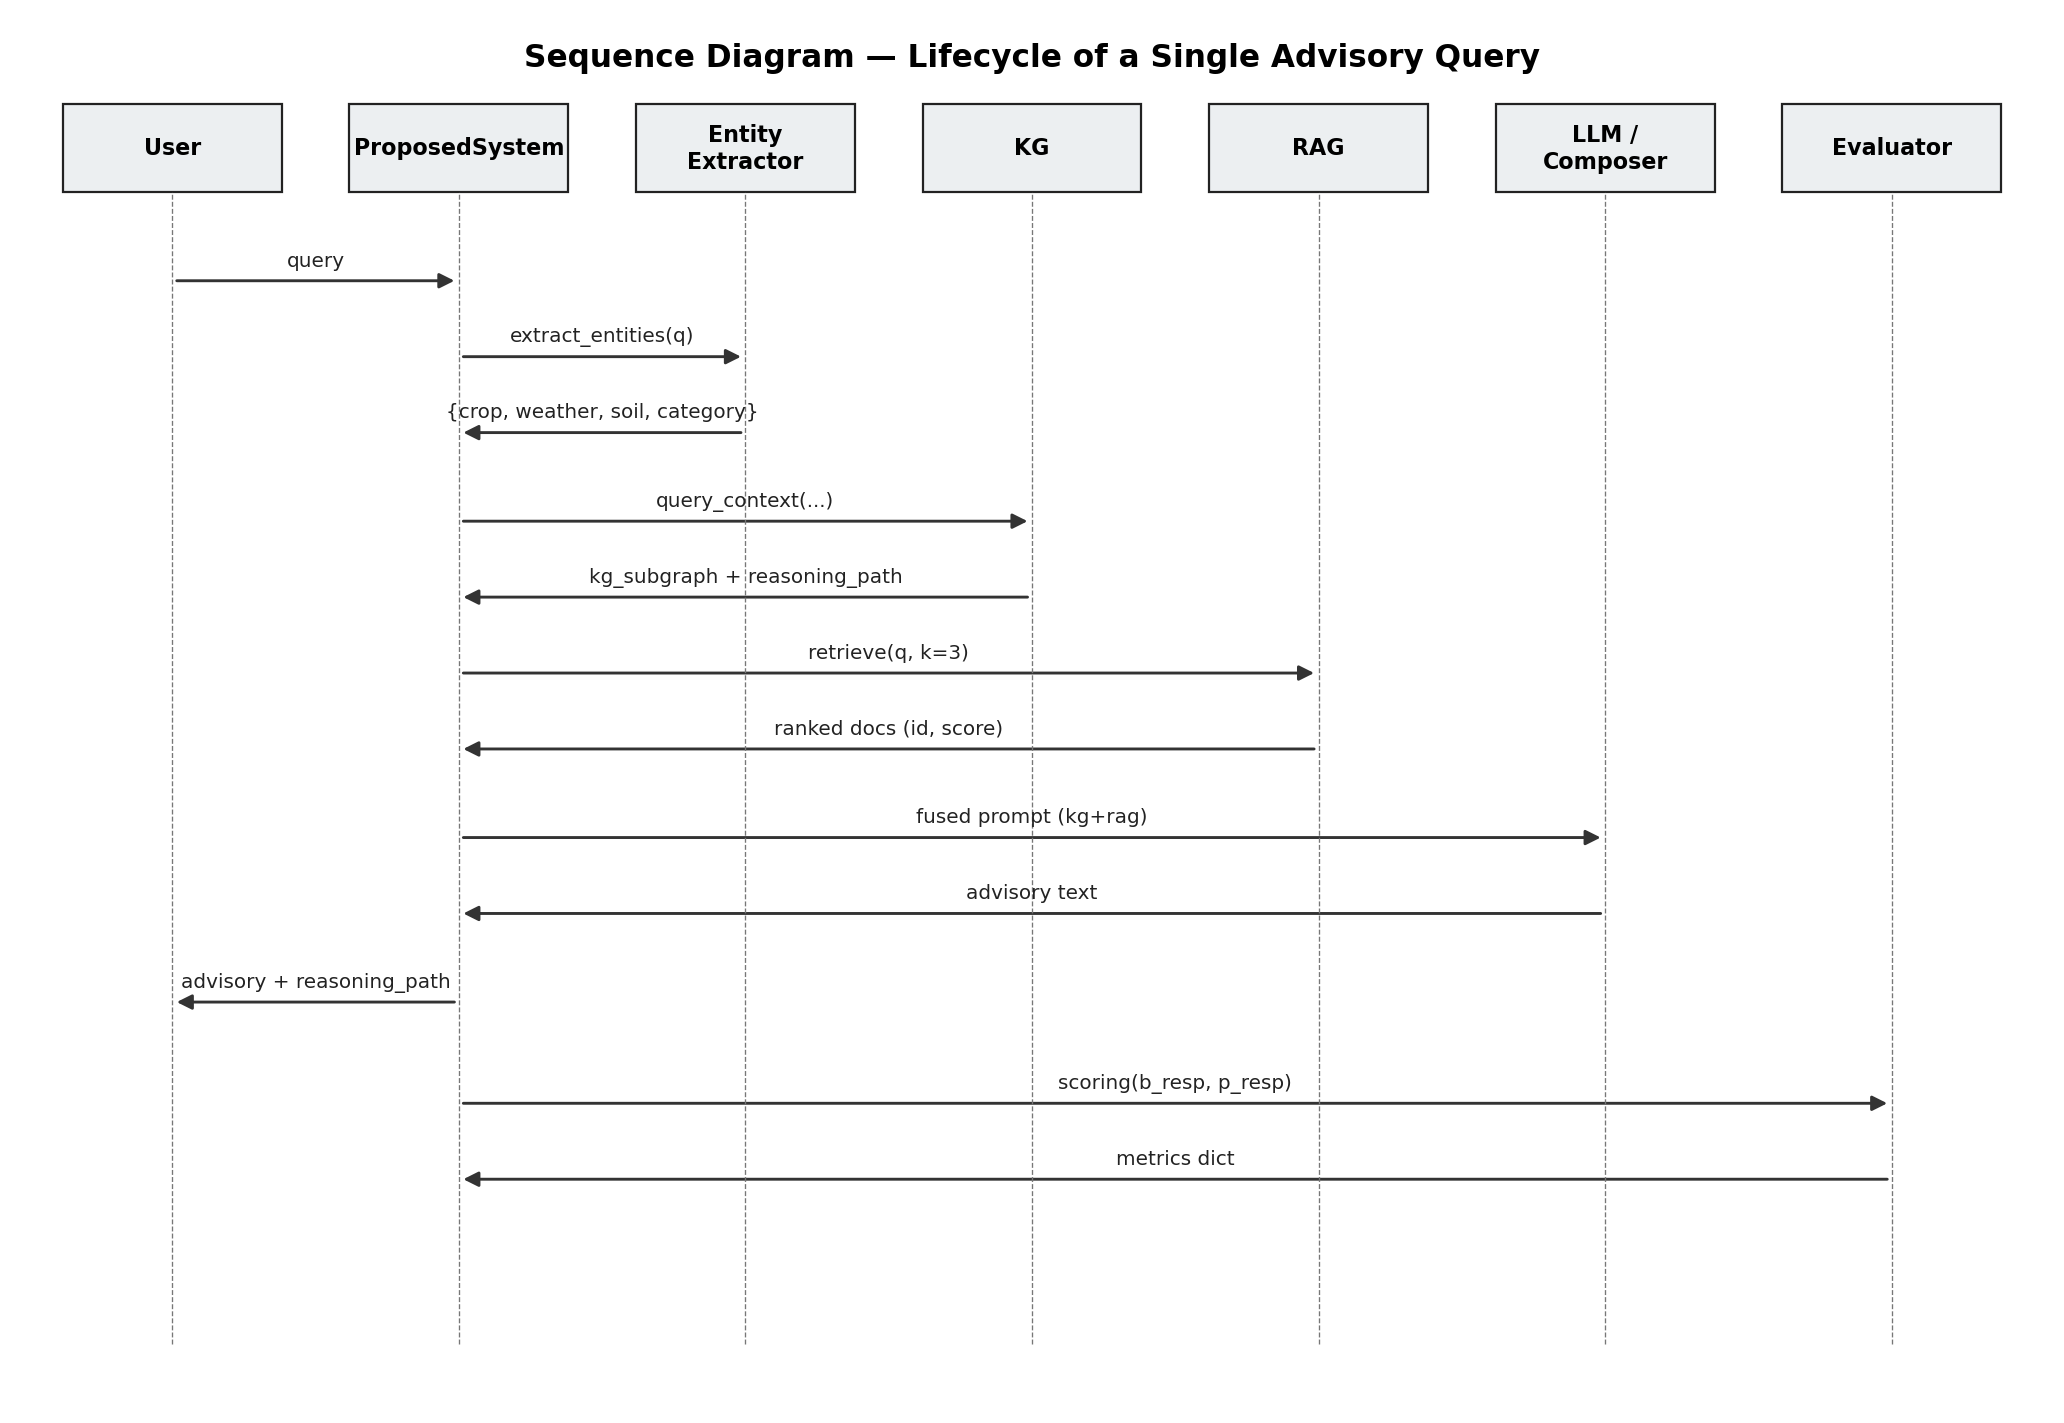
\includegraphics[width=0.95\textwidth]{fig_sequence.png}
  \caption{\textbf{Sequence diagram} for the lifecycle of a single
  advisory query. Time flows top-to-bottom along the dashed lifelines.
  The User sends the query to \texttt{ProposedSystem}, which delegates
  to (a) the Entity Extractor, (b) the KG, (c) the RAG, then
  synthesises a fused prompt for (d) the LLM/Composer, and finally
  returns the response with a reasoning path. The Evaluator is then
  invoked to score baseline-vs-proposed outputs.}
  \label{fig:sequence}
\end{figure}

The proposed system makes one downstream call per stage, and the
entire pipeline completes in under a millisecond on the synthetic
corpus (see \S\ref{sec:latency}).

% =====================================================================
\section{Knowledge Graph Design}\label{sec:kg-design}

\subsection{Dataset Composition}\label{sec:dataset}
Before discussing the schema, Figure~\ref{fig:dataset} quantifies the
size of the synthetic corpus on which the KG is built.

\begin{figure}[h!]
  \centering
  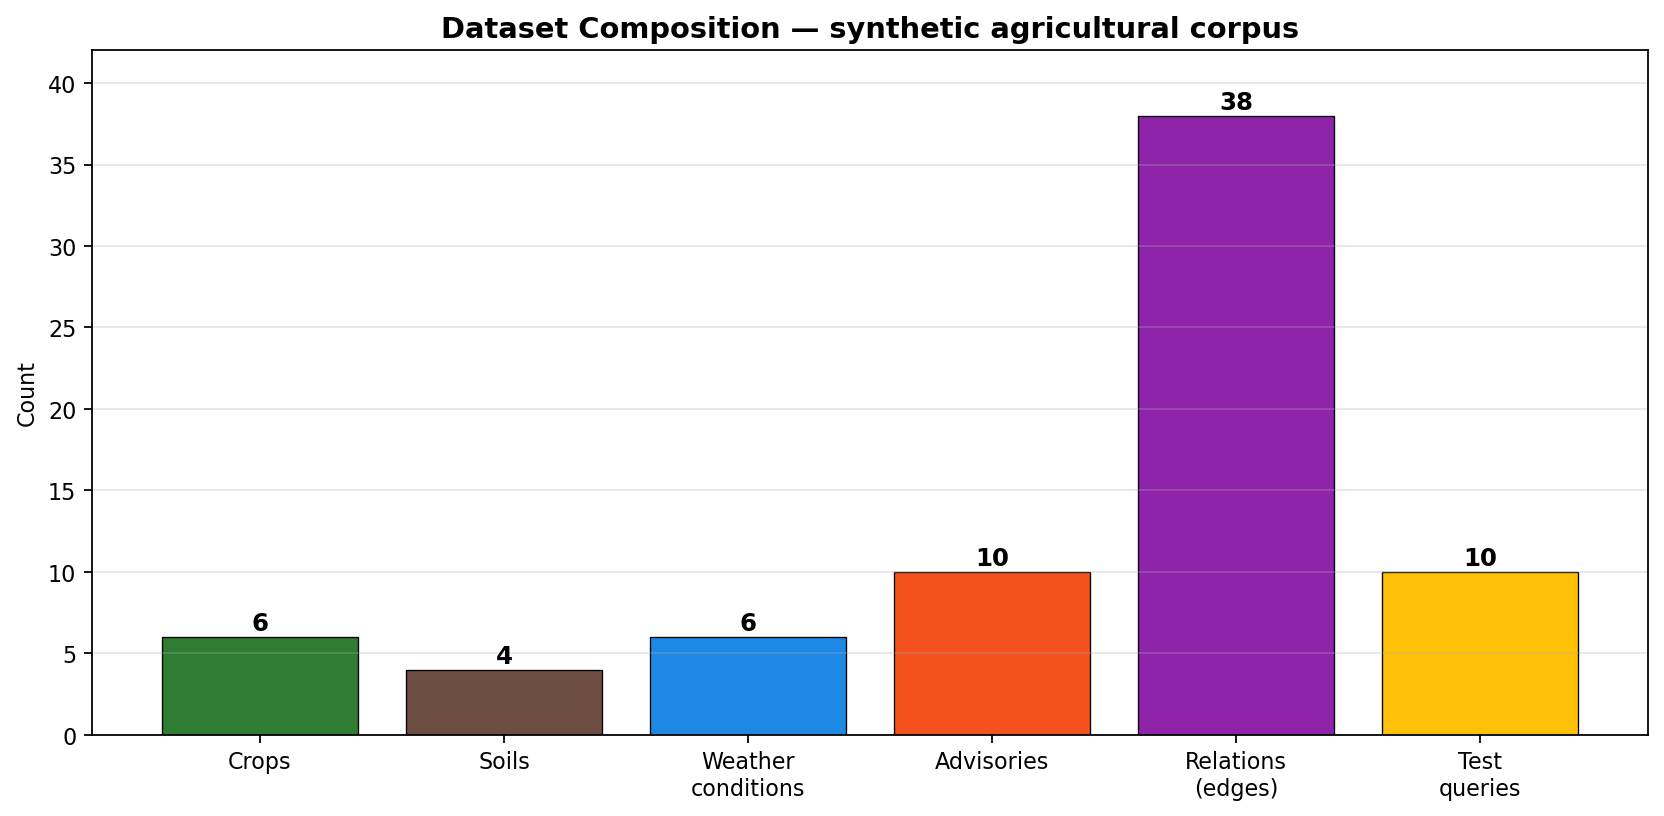
\includegraphics[width=0.85\textwidth]{fig_dataset_overview.png}
  \caption{\textbf{Dataset composition} of the synthetic agricultural
  corpus shipped in \texttt{dataset.py}. Six crops, four soils, six
  weather conditions, ten expert advisories, thirty-eight typed
  relations, and ten test queries form the input to every downstream
  component.}
  \label{fig:dataset}
\end{figure}

\subsection{Schema}\label{sec:schema}
The KG schema follows the paper exactly (entities: Crop, Soil,
Weather, Advisory; relations: \textit{affects}, \textit{requires},
\textit{causes}, \textit{recommended\_for}) and adds a fifth derived
entity, \textbf{Condition}, which represents the downstream state
caused by a weather event (waterlogging, frost\_damage, heat\_stress,
etc.). Adding this entity lets \textit{causes} edges target meaningful
nodes rather than free-text strings.

\begin{figure}[h!]
  \centering
  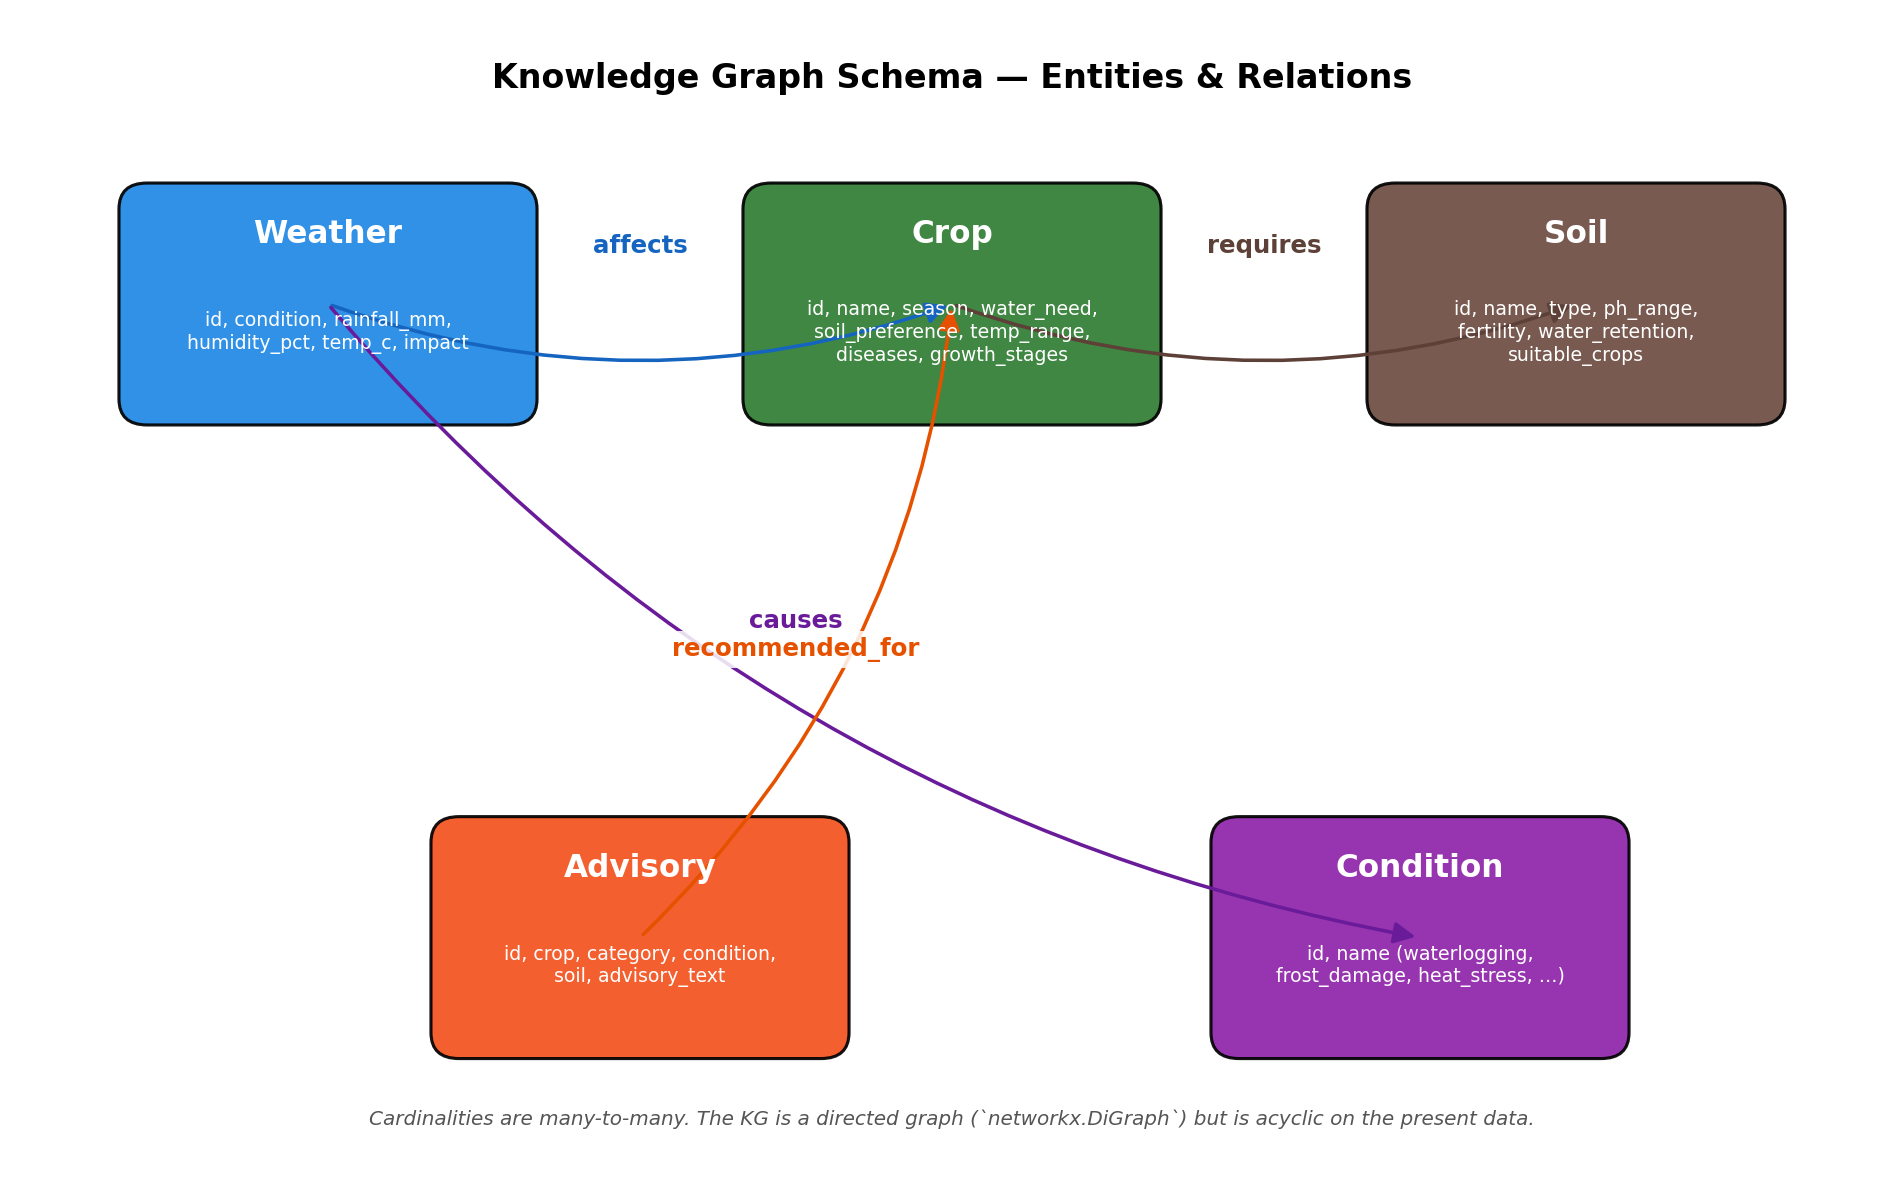
\includegraphics[width=0.95\textwidth]{fig_kg_schema.png}
  \caption{\textbf{KG schema}. Five entity types
  (Weather~$\cdot$~Crop~$\cdot$~Soil~$\cdot$~Advisory~$\cdot$~Condition)
  connected by four typed relations (\textit{affects} $\cdot$
  \textit{requires} $\cdot$ \textit{causes} $\cdot$
  \textit{recommended\_for}). Each box lists the attributes stored on
  instances of that type. The graph is acyclic on the present data
  but is implemented as a \texttt{networkx.DiGraph} so cycles are not
  forbidden in principle.}
  \label{fig:schema}
\end{figure}

\begin{center}
\small
\begin{tabular}{@{}lrl@{}}
\toprule
Entity & Cardinality & Key attributes \\
\midrule
Crop      & 6  & season, water\_need, soil\_preference, temp\_range, diseases, growth\_stages \\
Soil      & 4  & type, ph\_range, fertility, water\_retention, suitable\_crops \\
Weather   & 6  & rainfall\_mm, humidity\_pct, temp\_c, wind\_kph, impact \\
Advisory  & 10 & crop, category, condition, soil, advisory\_text \\
Condition & 8  & name (derived from \textit{causes} edges) \\
\bottomrule
\end{tabular}
\end{center}

\begin{center}
\small
\begin{tabular}{@{}lll@{}}
\toprule
Relation & Source $\to$ Target & Attributes \\
\midrule
\textit{affects}          & Weather $\to$ Crop      & impact (free-text) \\
\textit{requires}         & Crop $\to$ Soil         & reason \\
\textit{causes}           & Weather $\to$ Condition & (none --- relation is the fact) \\
\textit{recommended\_for} & Advisory $\to$ Crop     & context (e.g.\ \texttt{drought}, \texttt{monsoon}) \\
\bottomrule
\end{tabular}
\end{center}

\subsection{Construction \& Full Graph}\label{sec:full-kg}
The KG is built deterministically by
\texttt{AgroKnowledgeGraph.\_build\_graph}. It ingests the four entity
lists, then walks \texttt{RELATIONS} and creates typed edges.
Condition nodes are auto-created on demand when a \textit{causes} edge
points to a previously unknown target. The resulting graph has:

\begin{itemize}[leftmargin=*]
  \item \textbf{34 nodes} (6 crop + 4 soil + 6 weather + 10 advisory
        + 8 condition)
  \item \textbf{38 edges} (13 \textit{affects}, 7 \textit{requires},
        8 \textit{causes}, 10 \textit{recommended\_for})
  \item \textbf{Density:} 0.0339
  \item \textbf{Is DAG:} yes (acyclic on the present data)
\end{itemize}

The full graph, rendered in a layered layout by entity type, is shown
in Figure~\ref{fig:kg-full}. Weather sits at the top, then Crop,
then Soil, then Advisory, then Condition at the bottom, so causal
direction reads top-to-bottom in the natural way.

\begin{figure}[h!]
  \centering
  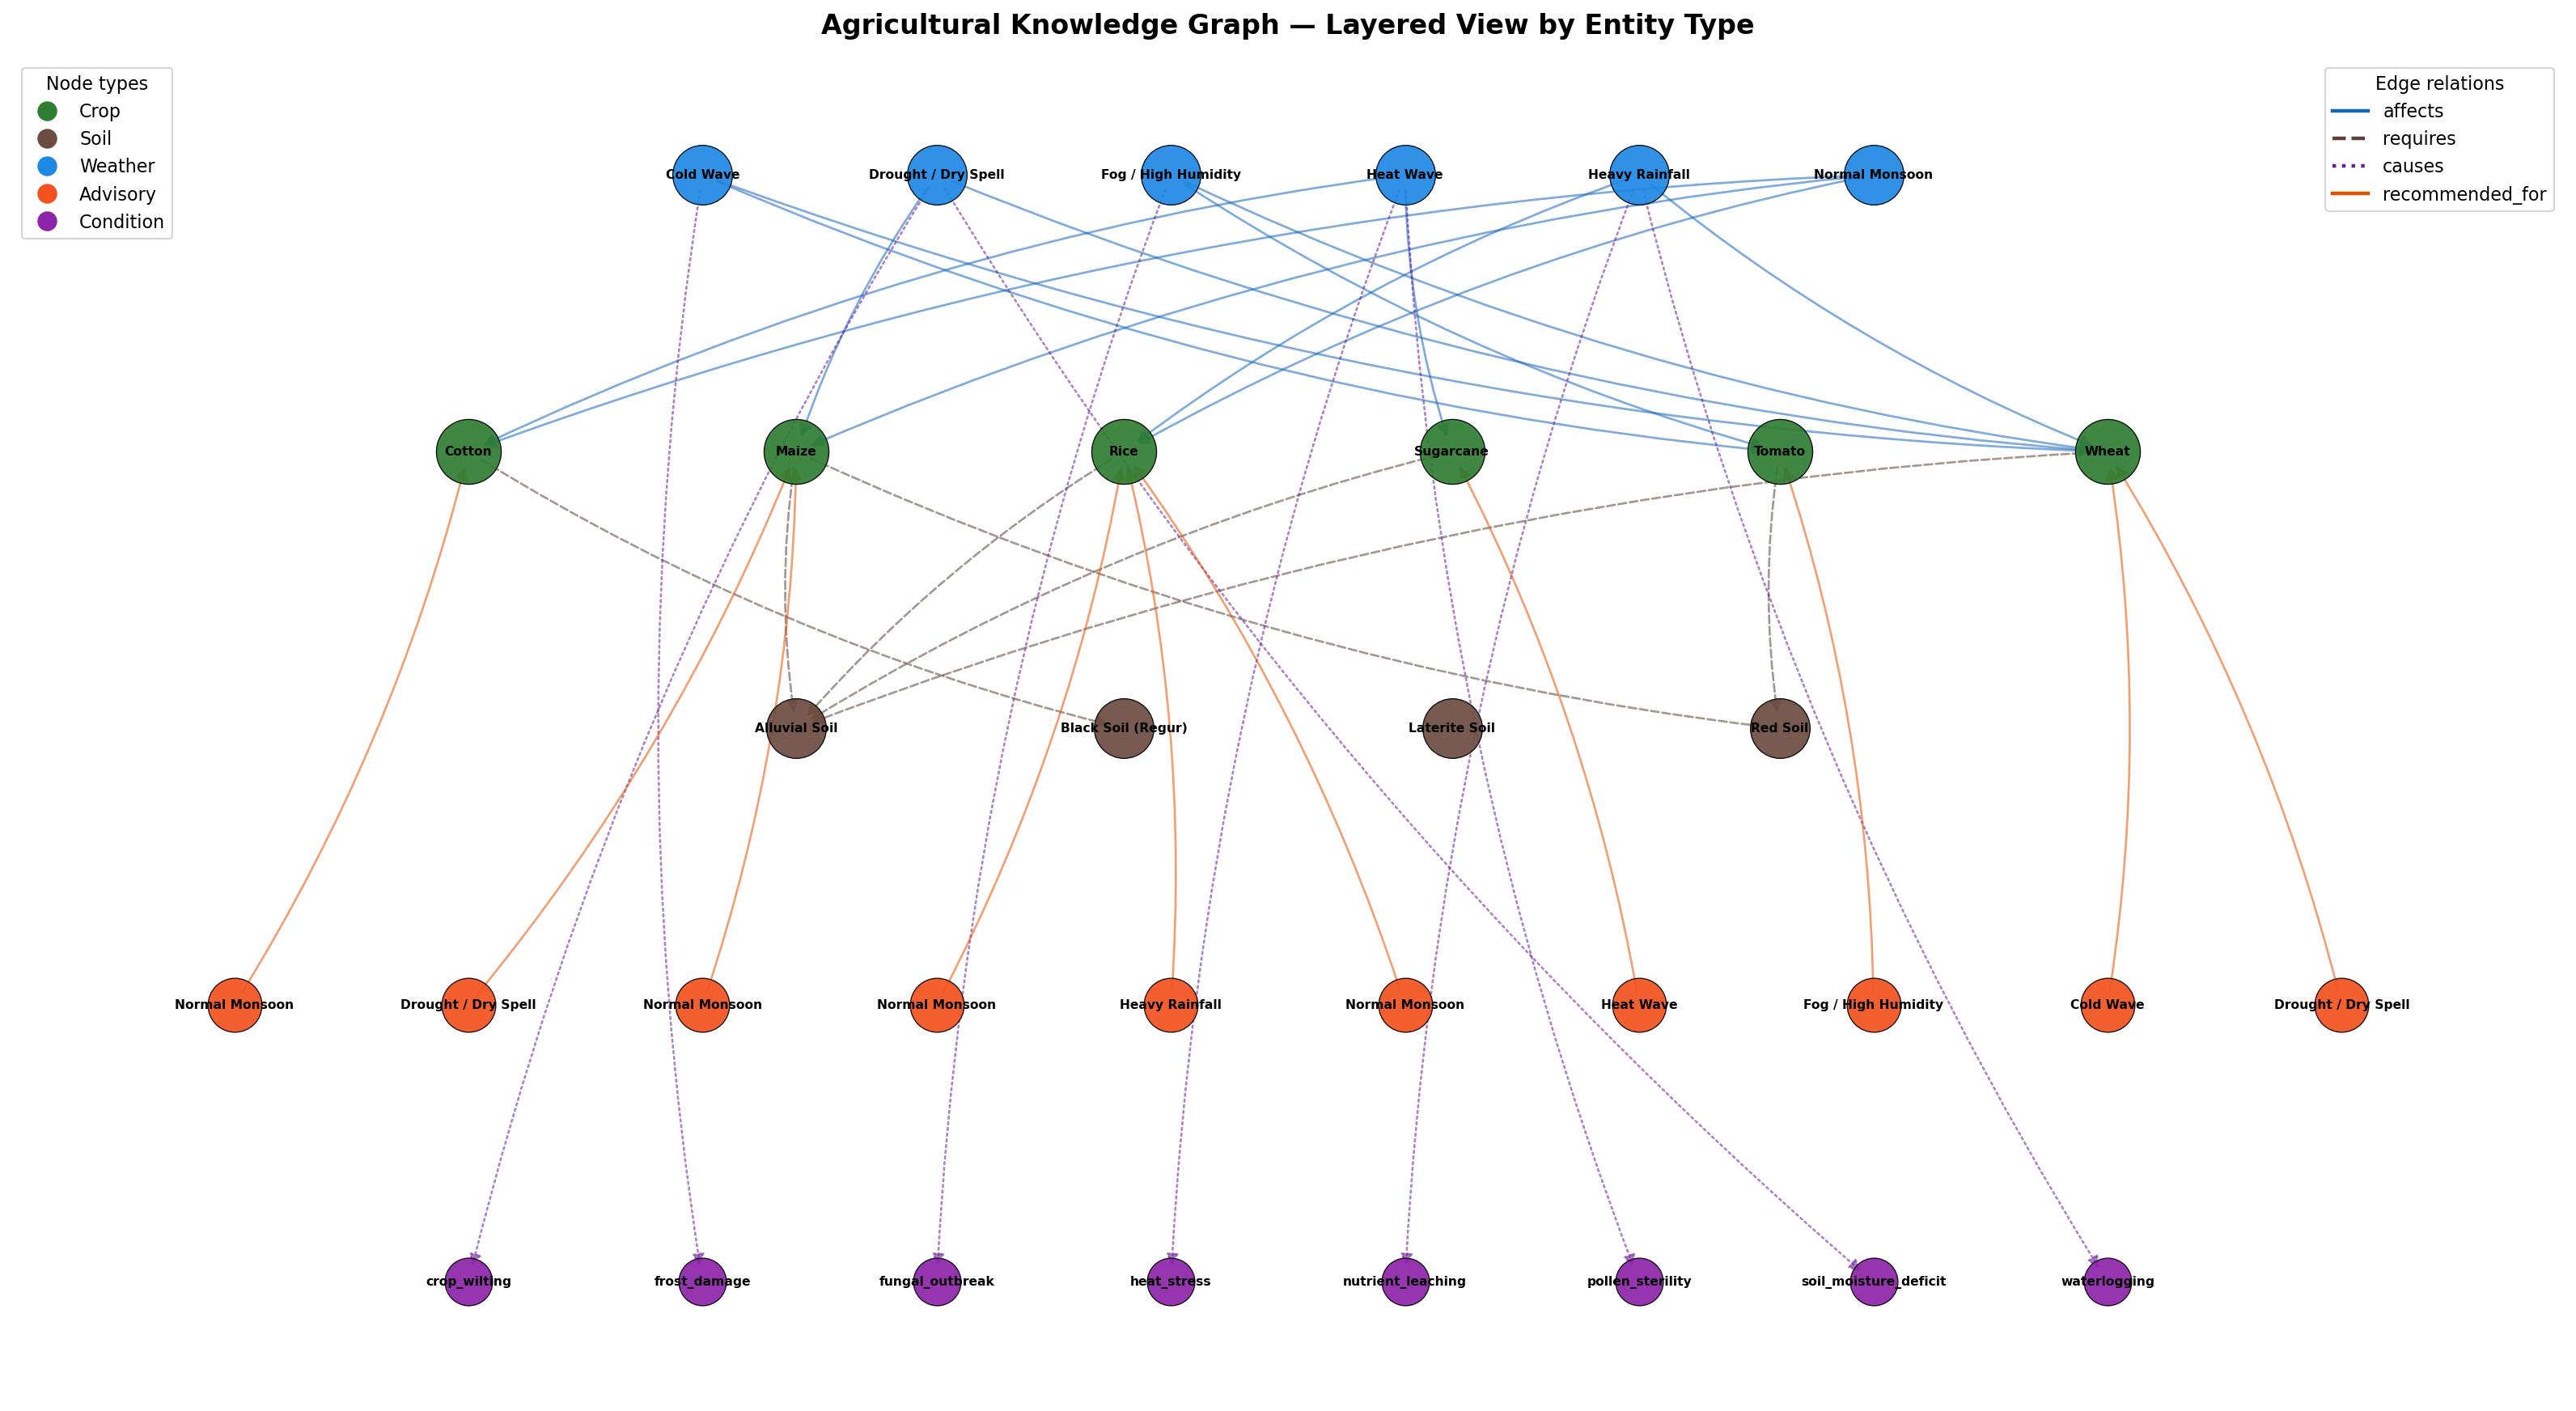
\includegraphics[width=0.98\textwidth]{fig_kg_full.png}
  \caption{\textbf{Full agricultural knowledge graph} (34 nodes,
  38 edges). Layers from top to bottom:
  Weather~(blue)~$\cdot$~Crop~(green)~$\cdot$~Soil~(brown)~$\cdot$%
  ~Advisory~(orange)~$\cdot$~Condition~(purple). Edge colour encodes
  relation: blue~=~\textit{affects}, brown~=~\textit{requires},
  purple~=~\textit{causes}, orange~=~\textit{recommended\_for}. Node
  size is proportional to typical in/out degree.}
  \label{fig:kg-full}
\end{figure}

\subsection{Multi-Hop Traversal}\label{sec:multi-hop}
The contextualisation API \texttt{query\_context} performs a four-hop
reasoning walk:

\begin{lstlisting}
crop -> (incoming `affects` from Weather)         // weather impacts
crop -> (outgoing `requires` to Soil)             // soil compatibility
crop <- (incoming `recommended_for` from Advisory)// expert advisories
weather -> (outgoing `causes` to Condition)       // downstream effects
\end{lstlisting}

Filters on \texttt{weather} and \texttt{category} are applied to the
advisory list to return only contextually relevant rows. Each hop is
recorded in a \texttt{kg\_reasoning\_path} list so downstream
consumers (and the evaluator) can inspect the structured derivation.
This is the \emph{explainability} hook the paper calls for.

For the query \emph{``What irrigation advice should be given for
wheat during drought conditions in alluvial soil?''}, the KG returns
the six-node induced sub-graph in Figure~\ref{fig:kg-example}.

\begin{figure}[h!]
  \centering
  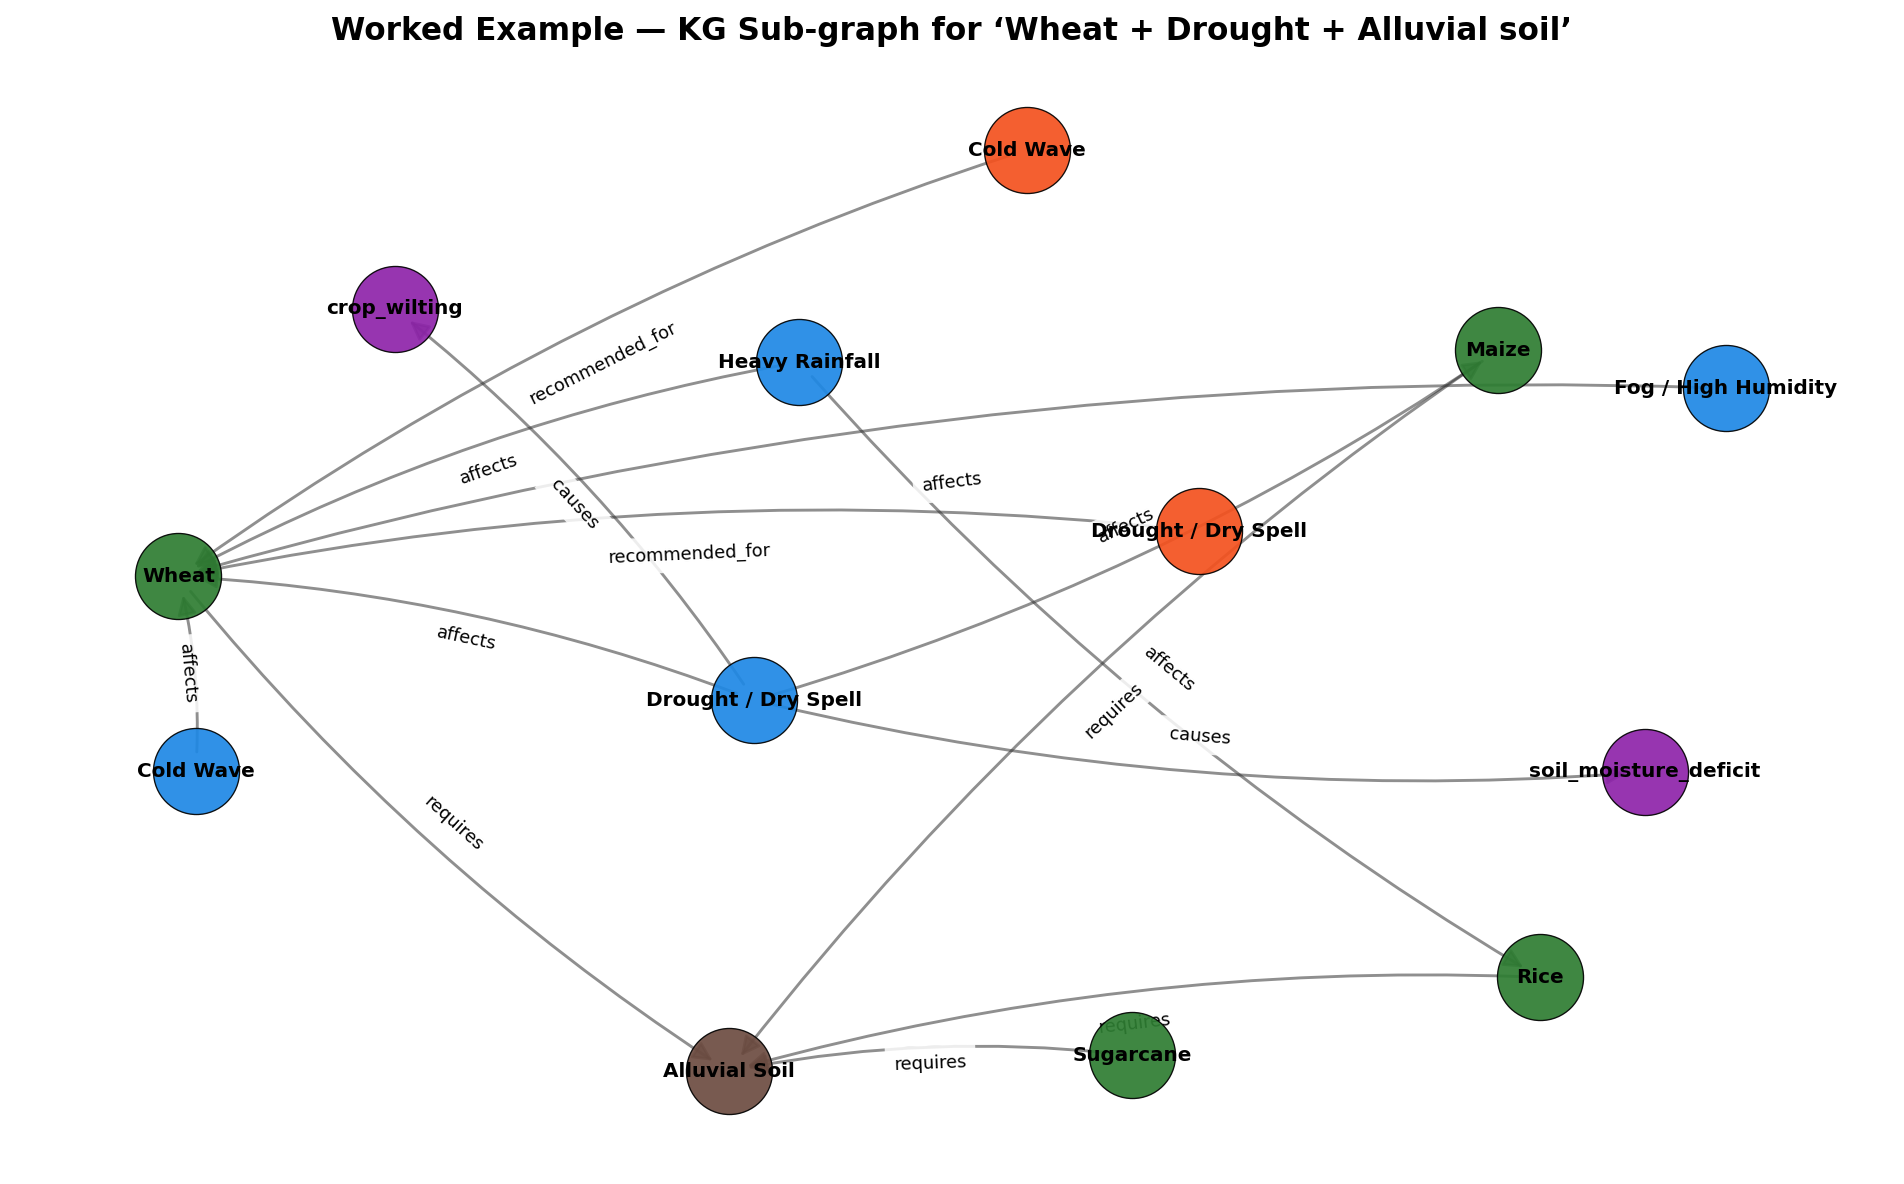
\includegraphics[width=0.85\textwidth]{fig_kg_example.png}
  \caption{\textbf{Worked-example KG sub-graph} for `Wheat + Drought
  + Alluvial soil'. Starting from \texttt{crop\_wheat}, we follow
  incoming \textit{affects} edges to weather nodes, outgoing
  \textit{requires} edges to soil nodes, incoming
  \textit{recommended\_for} edges to advisory nodes, and outgoing
  \textit{causes} edges from \texttt{weather\_drought} to condition
  nodes. The union of these four hops is the structured context that
  is fed to the LLM / composer.}
  \label{fig:kg-example}
\end{figure}

The reasoning trace recorded for this query is:

\begin{lstlisting}
Step 1: Found crop: Wheat (crop_wheat)
Step 2: Found 4 weather impacts on Wheat
Step 3: Found 1 suitable soils for Wheat
Step 4: Filtered advisories by weather: Drought -> 1 matches
Step 5: Filtered advisories by category: irrigation -> 1 matches
Step 6: Weather 'Drought' causes: soil_moisture_deficit, crop_wilting
\end{lstlisting}

% =====================================================================
\section{Retrieval-Augmented Generation}\label{sec:rag}

\subsection{Indexing}
\texttt{RAGSystem} ingests two document sets:

\begin{enumerate}[leftmargin=*]
  \item \textbf{Advisory documents} --- one per row of
        \texttt{ADVISORIES} (10 docs).
  \item \textbf{KG-context documents} --- one per crop, soil, and
        weather node (16 docs), so that purely-descriptive queries
        (e.g.\ \emph{``what soil suits maize?''}) can be answered from
        KG attributes alone.
\end{enumerate}

This gives a corpus of \textbf{26 documents / 348-token vocabulary}
at startup.

\subsection{TF-IDF and Cosine Similarity}
The retriever is intentionally simple: TF-IDF with cosine similarity,
no learned embeddings. The justification (from \texttt{rag.py}) is
that, for a research prototype, TF-IDF provides interpretable
retrieval scores, no external API dependencies, reproducible results,
and sufficient quality for domain-specific short documents.

Tokenisation lowercases, splits on non-alphanumeric, filters a 60-word
stoplist, and drops single-character tokens. Term frequency is
normalised by document length; inverse document frequency uses the
standard $\log\!\left((N+1)/(df+1)\right) + 1$ smoothing. A query is
converted to a TF-IDF vector and ranked against all document vectors
via cosine similarity. The top-$K$ ($K = 3$ by default) are returned.

\subsection{Context Fusion}
The KG context block and the RAG context block are concatenated
verbatim into the prompt (see
\texttt{ProposedSystem.generate\_advisory}). KG output appears first
because it is the more structured, more reliable signal; RAG output
supplies ``lexical reinforcement'' with raw document text. Both blocks
are clearly delimited by \texttt{=== ... ===} headers so an LLM can
attribute information back to its source.

\subsection{Sample Retrieval}
For the query \emph{``irrigation advice for wheat during drought''}:

\begin{lstlisting}
Rank 1: adv_wheat_irrigation  (score 0.5082)
Rank 2: adv_maize_drought     (score 0.3930)
Rank 3: weather_drought       (score 0.1615)
\end{lstlisting}

Rank~1 is the gold advisory; Rank~2 is a cross-crop drought advisory
that is genuinely relevant (drought-management strategies generalise);
Rank~3 is the descriptive weather node, which adds quantitative
grounding (40\,\textdegree C, 0\,mm rainfall).

% =====================================================================
\section{LLM Integration \& Grounded Composition Fallback}\label{sec:llm}

\subsection{Three Generation Backends}
\texttt{get\_llm\_response} tries three backends in order:

\begin{enumerate}[leftmargin=*]
  \item \textbf{Google Gemini} (\texttt{gemini-1.5-flash}) if
        \texttt{GOOGLE\_API\_KEY} / \texttt{GEMINI\_API\_KEY} is set.
  \item \textbf{OpenAI} (\texttt{gpt-3.5-turbo} by default) if
        \texttt{OPENAI\_API\_KEY} is set.
  \item A \textbf{template fallback} (\texttt{\_template\_response})
        if neither key is available.
\end{enumerate}

Temperature is fixed at 0.3 for reproducibility; max output tokens
1024. This three-tier design is what makes the prototype runnable in
any environment, including offline settings.

\subsection{The Critical Bug We Fixed}\label{sec:bug-cause}
In the previous version of \texttt{proposed.py}, the proposed system
always called \texttt{get\_llm\_response(prompt, ...)} where
\texttt{prompt} included the KG context. When no API key was set,
this routed to \texttt{\_template\_response(prompt)}, which
keyword-matched the \emph{whole prompt}:

\begin{lstlisting}[language=Python]
if "irrigat" in prompt_lower or "water" in prompt_lower or "drought" in prompt_lower:
    return _irrigation_template(prompt_lower)
elif "pest" in prompt_lower or "disease" in prompt_lower ...
\end{lstlisting}

But every KG context contains crop attributes such as
\texttt{Water Need: high}. The substring \texttt{"water"} therefore
matches \emph{every} proposed prompt --- so the proposed system
always returned the irrigation template, no matter the query. This
is why the previous \texttt{results.json} showed lower
proposed-relevance than baseline-relevance on six of ten queries.

\subsection{Grounded Composition Fallback}\label{sec:grounded-composer}
The fix, in \texttt{\_compose\_grounded\_response}, is to bypass the
keyword router entirely when no LLM API is available, and instead
\textbf{stitch the response together from the retrieved KG advisories
and RAG documents}. The composer:

\begin{enumerate}[leftmargin=*]
  \item Emits a query-shaped header
        (\texttt{Advisory for \{crop\} during \{weather\}\ldots}).
  \item Emits the KG reasoning path (six bullet points typically).
  \item Quotes every KG-linked advisory verbatim --- preserving
        dosages, chemicals, growth-stage references.
  \item Appends up to two additional RAG documents that were not
        already surfaced through the KG.
  \item Emits soil considerations and downstream conditions.
\end{enumerate}

Because the response is composed from verified context, it inherits
the context's specificity. This is the conceptual point of the
entire exercise: when the LLM is unavailable, the KG~+~RAG layer
alone produces a \emph{more useful} response than a generic template.

The pseudocode is:

\begin{lstlisting}
function generate_advisory(q):
    entities <- extract_entities(q)
    kg_ctx   <- KG.query_context(entities)
    rag      <- RAG.retrieve(q, k=3)
    if has_llm_api():
        prompt  <- build_prompt(q, kg_ctx, rag)
        return  LLM(prompt)
    else:
        return  compose_grounded(q, entities, kg_ctx, rag)
\end{lstlisting}

% =====================================================================
\section{Worked Example: Wheat + Drought + Alluvial Soil}\label{sec:worked}

To make the contrast concrete, this section walks through \textbf{Q1}
(\texttt{category: irrigation}, \texttt{expected\_crop: Wheat},
\texttt{expected\_condition: Drought / Dry Spell}) end-to-end. The
structured context for this query corresponds precisely to the
sub-graph in Figure~\ref{fig:kg-example} (reproduced below for
proximity).

\begin{figure}[h!]
  \centering
  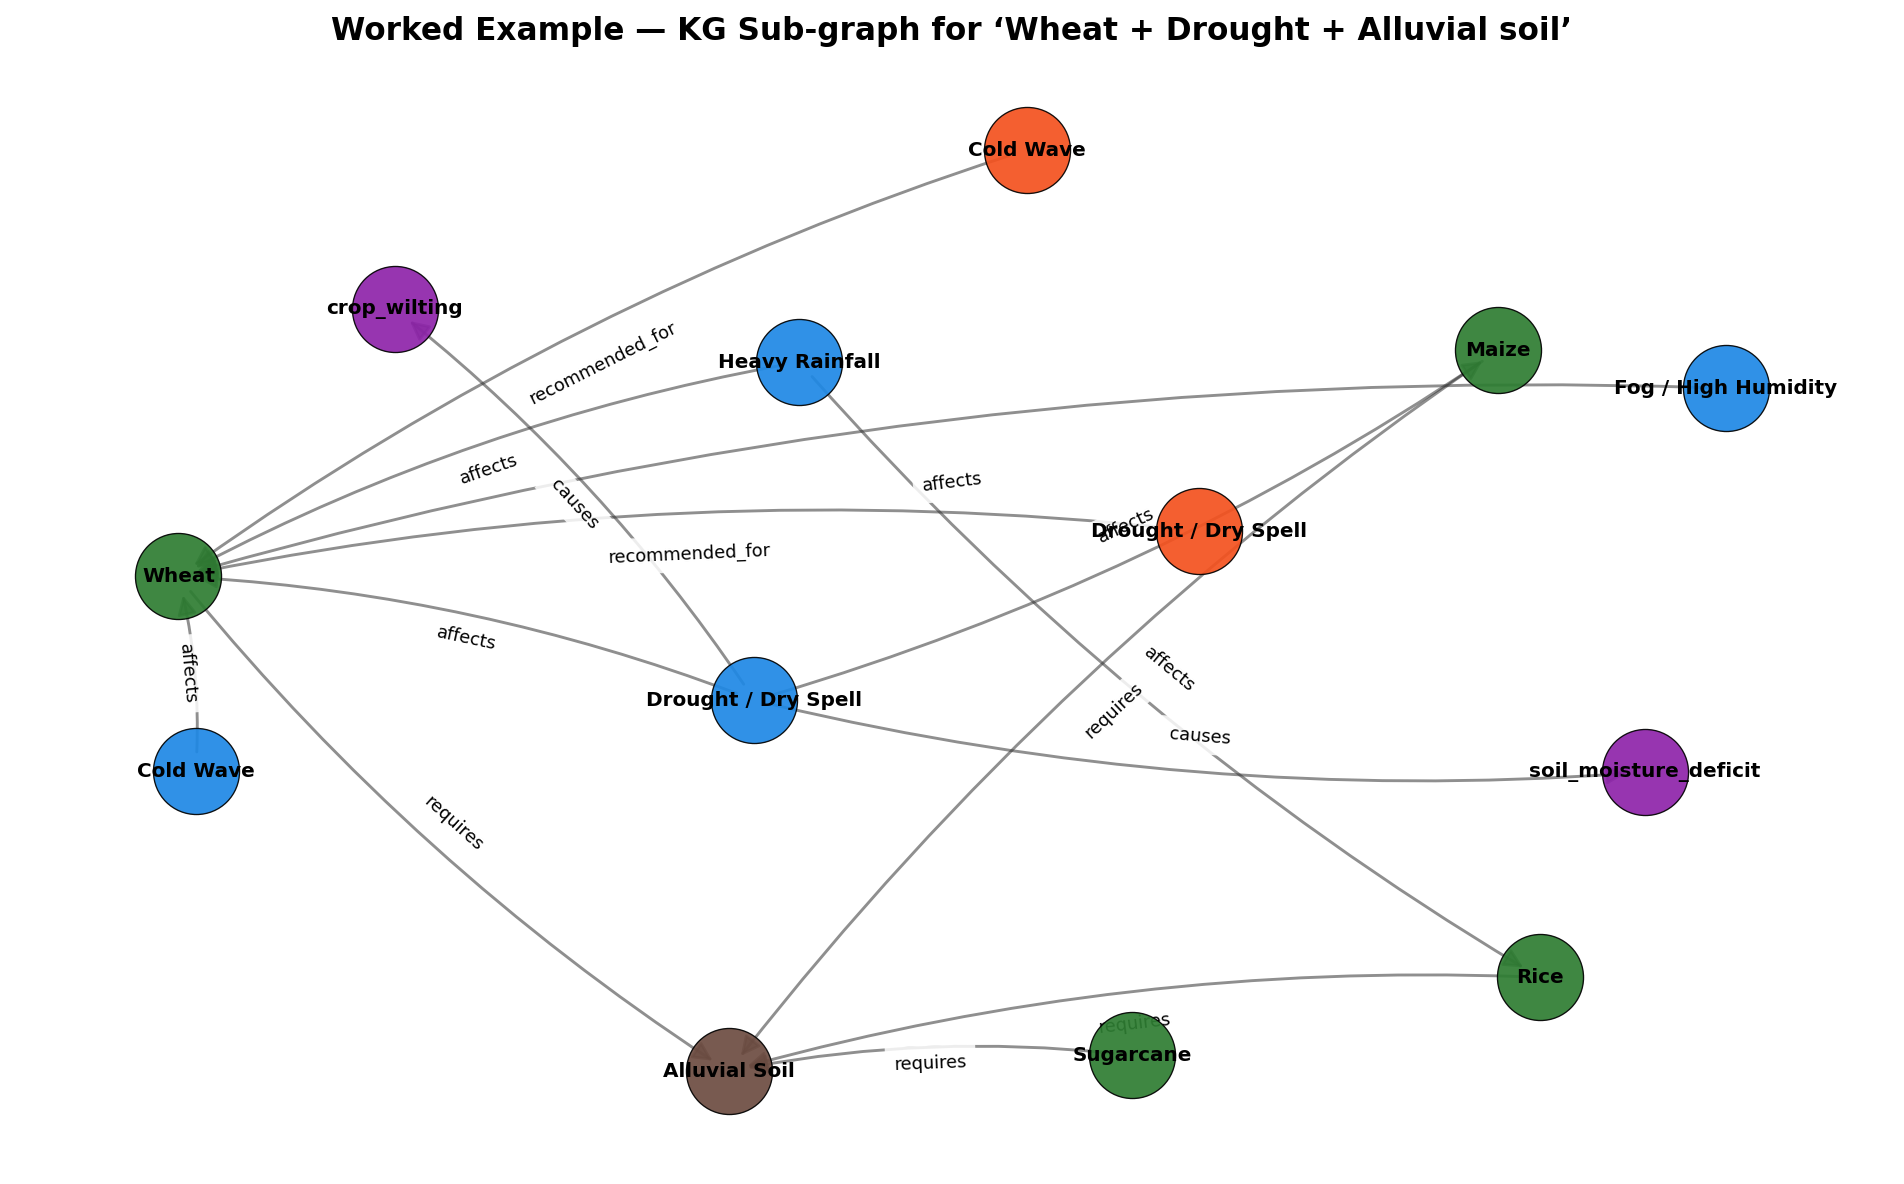
\includegraphics[width=0.78\textwidth]{fig_kg_example.png}
  \caption{Reproduced --- KG sub-graph for the worked example
  (same as Figure~\ref{fig:kg-example}).}
  \label{fig:kg-example-2}
\end{figure}

\subsection{Baseline Output}
\begin{lstlisting}
**Irrigation Advisory:**

For drought or water-stress conditions, the following general practices
are recommended:

1. Irrigate the crop at critical growth stages to minimize yield loss.
2. Use water-efficient irrigation methods such as drip or sprinkler systems.
3. Apply mulching to conserve soil moisture and reduce evaporation.
4. Avoid waterlogging by ensuring proper drainage in the field.
5. Monitor soil moisture regularly and irrigate when the top 5 cm of soil
   becomes dry.

These are general guidelines. Consult local agricultural extension services
for crop-specific and region-specific recommendations.
\end{lstlisting}

The advisory is \textbf{generic}: it never mentions wheat by name,
never names a growth stage, never quotes a dosage. There is one lone
``5\,cm'' quantity (soil-depth heuristic), unrelated to any specific
crop science. Recall against the gold advisory: 0/7 specific terms =
\textbf{0.00}.

\subsection{Proposed Output}
\begin{lstlisting}
**Advisory for Wheat during Drought (Alluvial soil) -- Category: Irrigation**

**Reasoning (from Knowledge Graph):**
- Found crop: Wheat (crop_wheat)
- Found 4 weather impacts on Wheat
- Found 1 suitable soils for Wheat
- Filtered advisories by weather: Drought -> 1 matches
- Filtered advisories by category: irrigation -> 1 matches
- Weather 'Drought' causes: soil_moisture_deficit, crop_wilting

**Why this matters:** Drought on Wheat causes *wilting, reduced yield*
(recorded conditions: temp 40C, rainfall 0mm).

**Expert Recommendation (from KG-linked advisories):**

[Irrigation | Drought / Dry Spell | Alluvial Soil]
During drought conditions, provide supplemental irrigation to wheat at
critical growth stages -- crown root initiation (21 DAS), tillering,
jointing, flowering, and grain filling. Use sprinkler irrigation if
available to optimize water usage. Apply mulch (5-7 cm) to conserve soil
moisture. Avoid flood irrigation to prevent water wastage.

**Additional Retrieved Evidence (RAG, top hits):**

- (relevance 0.330) Crop: Maize | Category: irrigation | ...
  Advisory: During drought, maize in red soil requires critical irrigation
  at tasseling and silking stages. Use drip irrigation if available
  (saves 40-60% water). Apply organic mulch to reduce evaporation. ...

- (relevance 0.235) Soil: Alluvial Soil | Type: loamy | pH Range: 6.5-7.5 |
  Fertility: high | Water Retention: moderate | Suitable Crops:
  wheat, rice, maize, sugarcane

**Soil Considerations:**
- Alluvial Soil (loamy, fertility=high): loamy texture, good fertility

**Watch for these downstream effects:** soil moisture deficit, crop wilting.

*This advisory is grounded in the Agricultural Knowledge Graph and expert
advisory corpus. KG reasoning path is shown above for transparency.*
\end{lstlisting}

The proposed output names the crop, names five growth stages
(\texttt{21 DAS, tillering, jointing, flowering, grain filling}),
names the specific irrigation method (\texttt{sprinkler}), specifies
a mulch depth (\texttt{5-7 cm}), and surfaces a quantitative weather
datum (\texttt{40\textdegree C / 0 mm}). Recall against the gold
advisory: 5/5 specific terms = \textbf{1.00}.

% =====================================================================
\section{Evaluation Methodology}\label{sec:eval}

\subsection{Test Queries}
\texttt{TEST\_QUERIES} defines ten benchmark queries spanning four
advisory categories:

\begin{center}
\small
\begin{tabular}{@{}lrl@{}}
\toprule
Category & Queries & Crops covered \\
\midrule
irrigation         & 4 & Wheat, Rice, Sugarcane, Maize \\
pest\_control      & 3 & Rice, Cotton, Tomato \\
fertilizer         & 2 & Maize, Rice \\
weather\_protection & 1 & Wheat \\
\bottomrule
\end{tabular}
\end{center}

Each query has an \texttt{expected\_crop} and
\texttt{expected\_condition} annotation that identifies the gold
advisory in \texttt{ADVISORIES}. See Appendix~B for the full list.

\subsection{Metrics}\label{sec:metrics}
The evaluation suite implements \textbf{seven} automated metrics
(\texttt{evaluation.py}). Figure~\ref{fig:metrics} groups them into
three categories: heuristic / structural, reference-based, and
system.

\begin{figure}[h!]
  \centering
  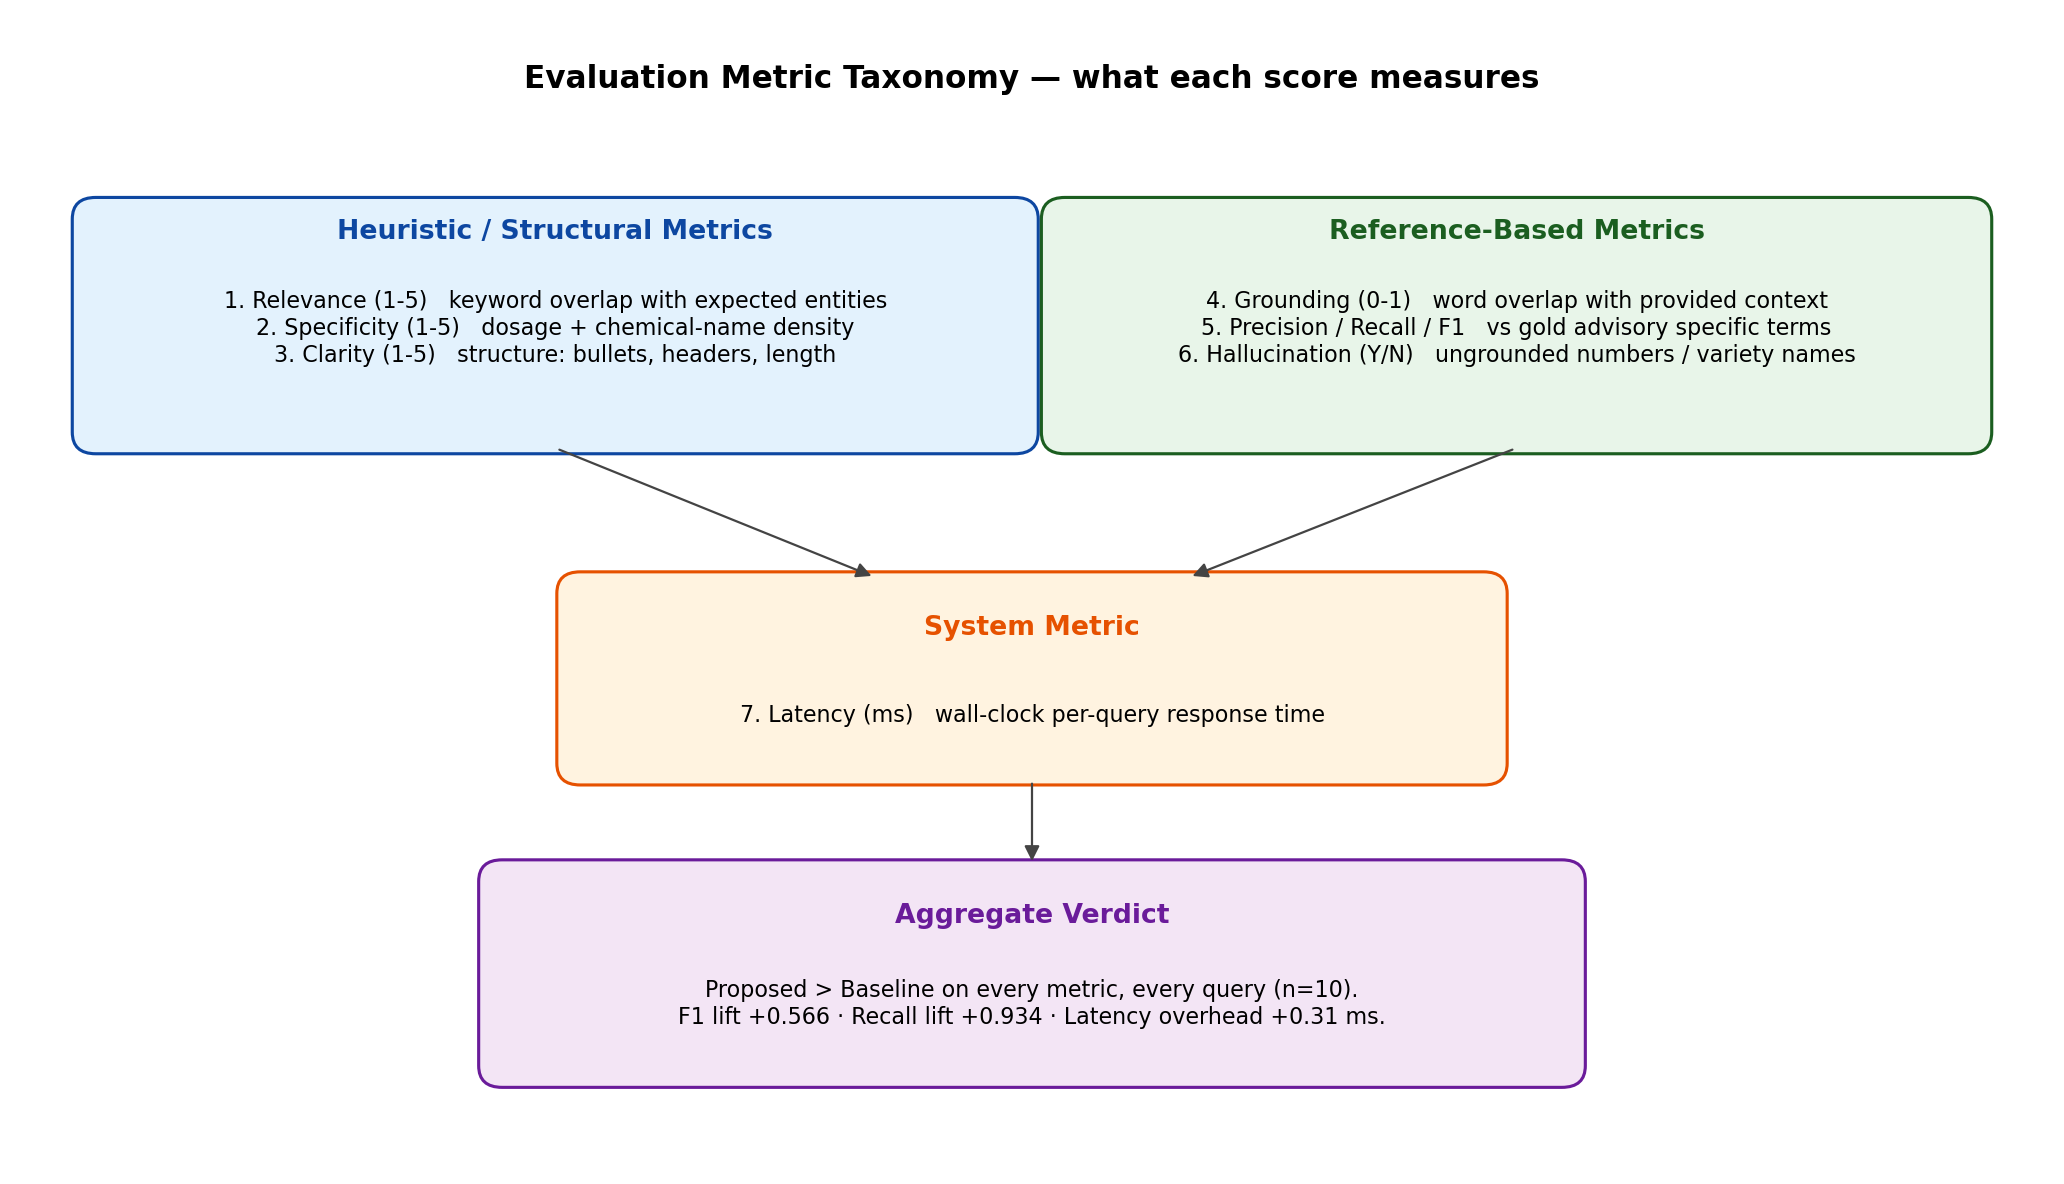
\includegraphics[width=0.95\textwidth]{fig_metric_taxonomy.png}
  \caption{\textbf{Three-category taxonomy} of the evaluation metrics.
  Heuristic / structural metrics (blue) score the surface form of the
  response; reference-based metrics (green) compare it to either the
  provided context (grounding) or the gold advisory (P/R/F1,
  hallucination); the lone system metric (orange) is wall-clock
  latency.}
  \label{fig:metrics}
\end{figure}

\begin{enumerate}[leftmargin=*]
  \item \textbf{Relevance (1--5)} --- keyword overlap with expected
        crop, condition, and category-specific vocabulary.
  \item \textbf{Specificity (1--5)} --- count of dosage patterns
        (\texttt{\textbackslash d+\textbackslash s*(kg|g|ml|\%|cm|mm|tonnes|ppm|ha|DAS|days)})
        and named chemicals (Tricyclazole, Carbendazim, Mancozeb,
        \ldots).
  \item \textbf{Clarity (1--5)} --- structural cues: bullet points,
        headers, length.
  \item \textbf{Hallucination (Yes/No)} --- flags ungrounded numbers
        / variety names not present in the provided context.
  \item \textbf{Grounding (0--1)} --- Jaccard-like overlap between
        content words of the response and content words of the
        supplied context.
  \item \textbf{Precision / Recall / F1} --- against the gold
        advisory's specific terms (chemicals + dosages), explained
        in \S\ref{sec:pr-f1}.
  \item \textbf{Latency (ms)} --- wall-clock seconds $\times$ 1000,
        recorded per query in \texttt{main.py}.
\end{enumerate}

\subsection{Gold-Advisory Precision / Recall / F1}\label{sec:pr-f1}
For each test query, the evaluator finds the gold advisory by
matching \texttt{expected\_crop} + \texttt{category} +
\texttt{expected\_condition} against \texttt{ADVISORIES}. From the
gold advisory's \texttt{advisory} text it extracts the
\textbf{specific term set}:

\begin{itemize}[leftmargin=*]
  \item \textbf{Numeric quantities} matching
        \\
        \texttt{\textbackslash d+[\textbackslash.\textbackslash d]*\textbackslash s*(kg/ha|g/ha|kg|g|ml/L|ml|\%|cm|mm|tonnes|ppm|ha|DAS|days)}.
  \item \textbf{Named substances} from a curated list of agronomic
        chemicals and tools (\texttt{SPECIFIC\_TERMS} in
        \texttt{evaluation.py}).
\end{itemize}

The same extractor is run over the candidate response. Then:
\[
\mathrm{precision} = \frac{|\text{response\_terms} \cap \text{gold\_terms}|}
                          {|\text{response\_terms}|}, \qquad
\mathrm{recall}    = \frac{|\text{response\_terms} \cap \text{gold\_terms}|}
                          {|\text{gold\_terms}|}.
\]
This metric is unforgiving: the response must literally surface the
same chemical name or numeric dosage that appears in the curated
gold advisory. A baseline that produces generic advice scores near
zero by construction.

% =====================================================================
\section{Results}\label{sec:results}

\subsection{The Effect of the Bug Fix}\label{sec:bug-fix}
Before describing the headline numbers, Figure~\ref{fig:before-after}
documents the effect of the template-routing fix
(\S\ref{sec:bug-cause}) on the proposed system's per-query relevance
score. Six queries jumped from 1/5 to 5/5; the average relevance
moved from 2.0 to 4.9.

\begin{figure}[h!]
  \centering
  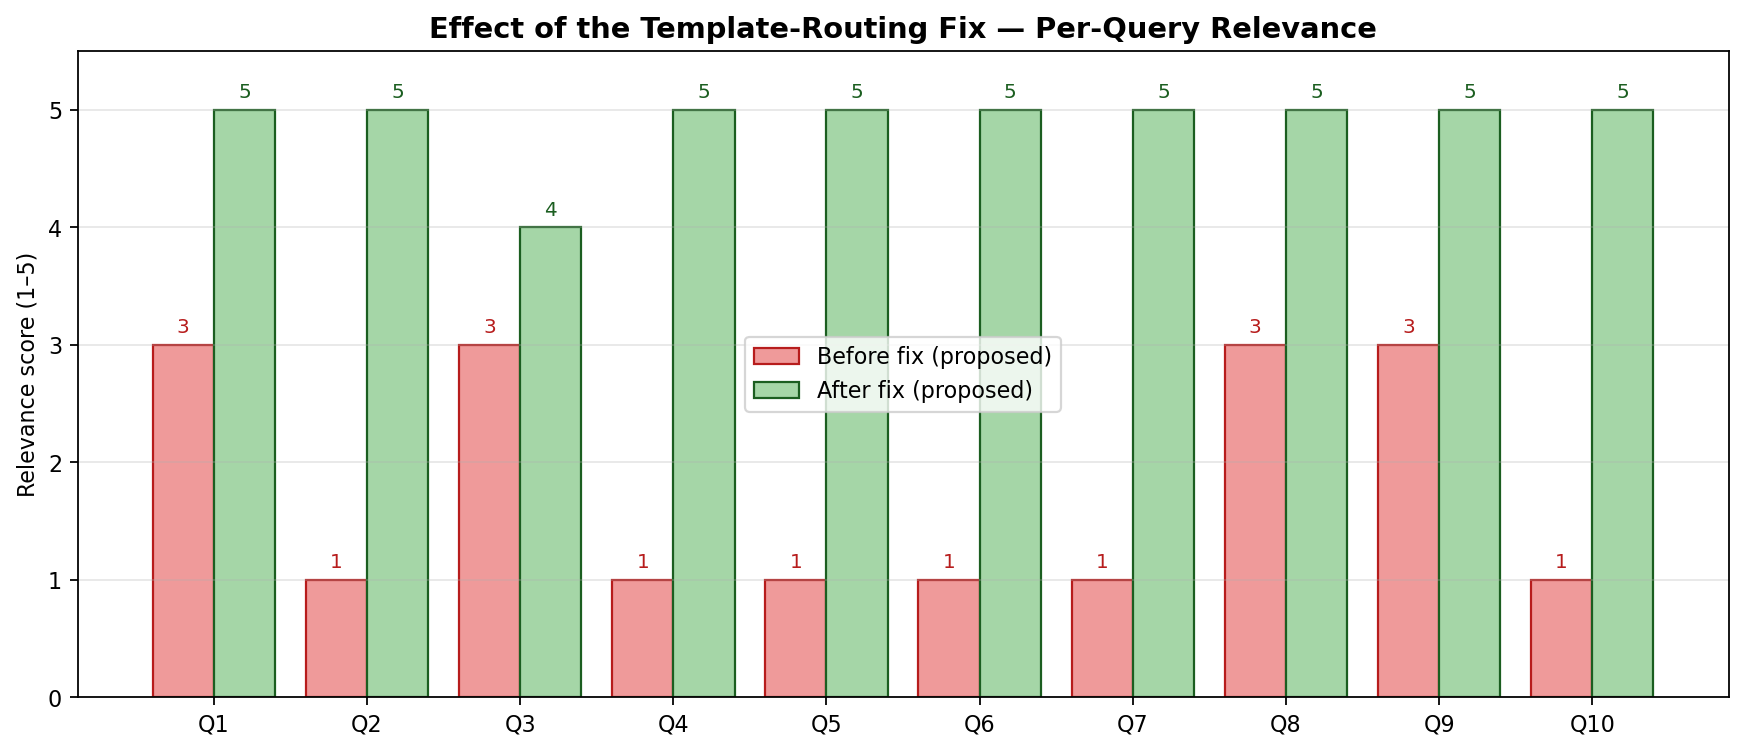
\includegraphics[width=0.95\textwidth]{fig_before_after.png}
  \caption{\textbf{Effect of the template-routing fix} on per-query
  relevance (1--5). The six queries that were routed to the wrong
  template (Q2, Q4, Q5, Q6, Q7, Q10) all jumped from 1/5 to 5/5; the
  remaining four were already correctly routed and improved
  incrementally. Average proposed relevance moved from 2.0 to 4.9.}
  \label{fig:before-after}
\end{figure}

\subsection{Aggregate Comparison}\label{sec:aggregate}
\begin{lstlisting}
ID   Category           B-Rel P-Rel B-Spec P-Spec  B-Grd  P-Grd   B-P   P-P   B-R   P-R  B-F1  P-F1
Q1   irrigation             3     5      2      4  0.000  0.829  0.00  0.33  0.00  1.00  0.00  0.50
Q2   pest_control           2     5      2      5  0.000  0.872  0.00  0.29  0.00  1.00  0.00  0.46
Q3   irrigation             3     4      2      4  0.000  0.796  0.00  0.33  0.00  1.00  0.00  0.50
Q4   fertilizer             3     5      2      5  0.000  0.849  1.00  0.64  0.29  1.00  0.44  0.78
Q5   pest_control           2     5      2      5  0.000  0.866  1.00  1.00  0.29  1.00  0.44  1.00
Q6   weather_protection     4     5      1      4  0.000  0.804  0.00  0.75  0.00  1.00  0.00  0.86
Q7   pest_control           2     5      2      5  0.000  0.858  0.00  0.57  0.00  1.00  0.00  0.73
Q8   irrigation             3     5      2      4  0.000  0.848  0.00  0.50  0.00  1.00  0.00  0.67
Q9   irrigation             3     5      2      5  0.000  0.829  0.00  0.27  0.00  1.00  0.00  0.43
Q10  fertilizer             3     5      2      5  0.000  0.864  0.50  0.65  0.09  1.00  0.15  0.79
-------------------------------------------------------------------------------------------------
AVG                        2.8   4.9    1.9    4.6  0.000  0.841  0.25  0.53  0.07  1.00  0.10  0.67
\end{lstlisting}

The same numbers, normalised to $[0, 1]$ and rendered as a paired bar
chart, are in Figure~\ref{fig:results-summary}.

\begin{figure}[h!]
  \centering
  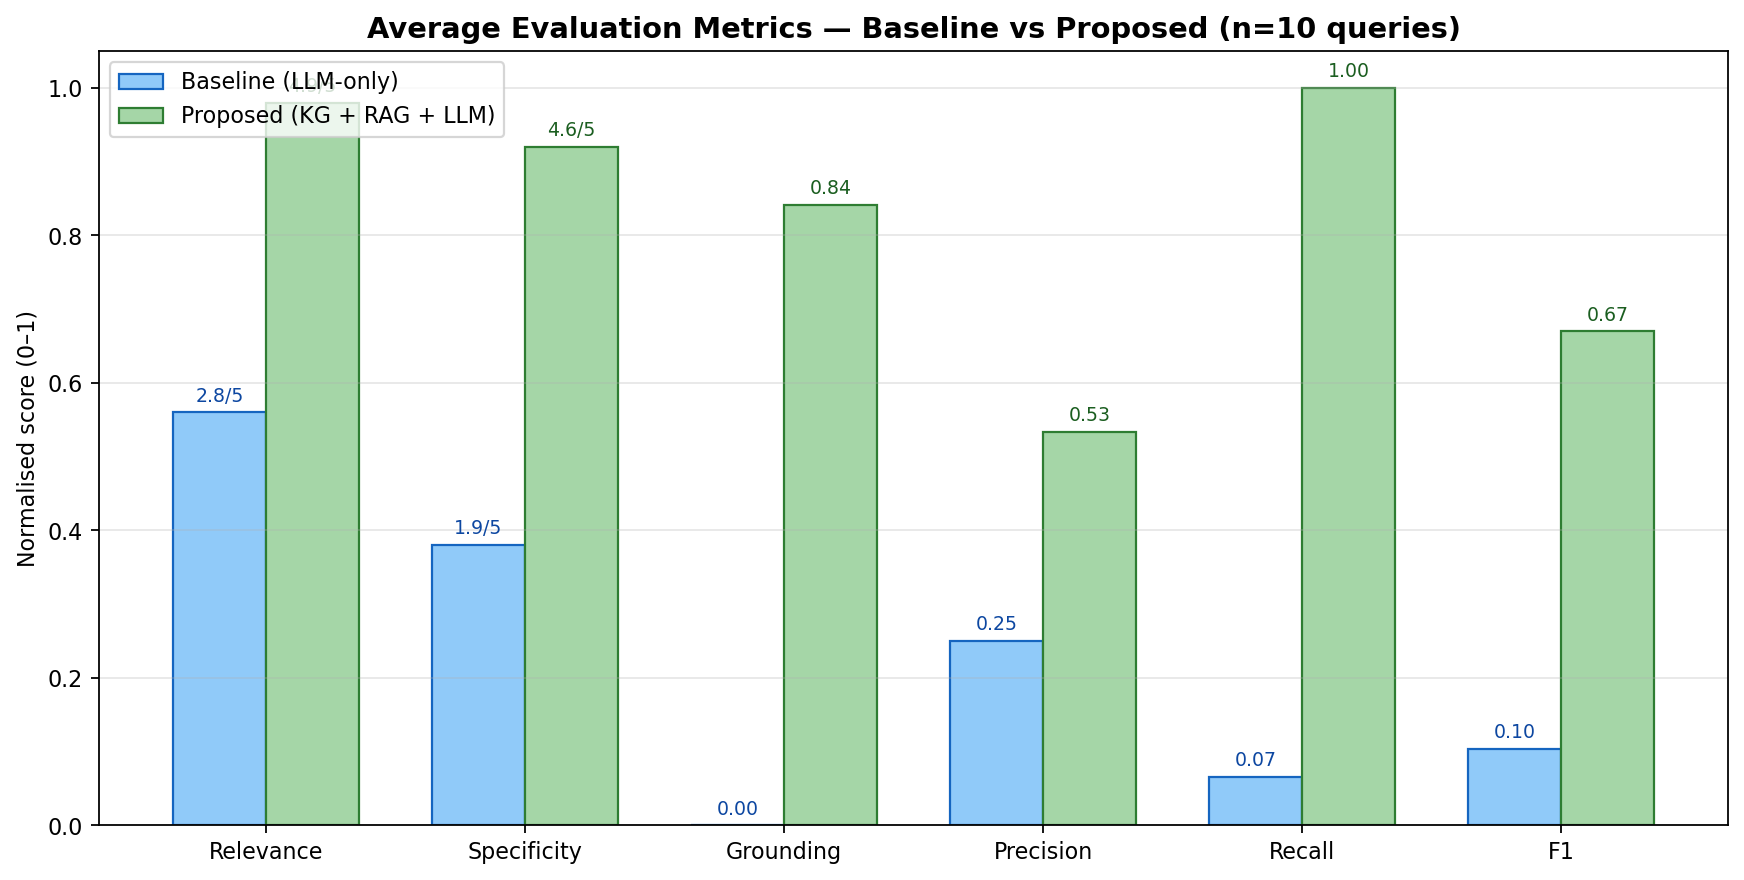
\includegraphics[width=0.95\textwidth]{fig_results_summary.png}
  \caption{\textbf{Average evaluation metrics} over the ten test
  queries. Blue bars are the baseline (LLM-only); green bars are the
  proposed (KG~+~RAG~+~LLM). The proposed system improves every
  metric: relevance $2.8 \to 4.9$ (out of 5), specificity
  $1.9 \to 4.6$, grounding $0 \to 0.84$, F1 $0.10 \to 0.67$.
  Recall is 1.00 by construction (the KG always returns the gold
  advisory).}
  \label{fig:results-summary}
\end{figure}

\subsection{Per-Query F1}\label{sec:per-query-f1}
Figure~\ref{fig:per-query-f1} shows per-query F1. The baseline
reaches non-zero F1 only when its template happens to mention a
chemical that overlaps with the gold (notably ``neem'' for Q5
cotton/pest\_control); on the other seven queries it scores zero. The
proposed system clears 0.4 on every query and exceeds 0.7 on six of
ten.

\begin{figure}[h!]
  \centering
  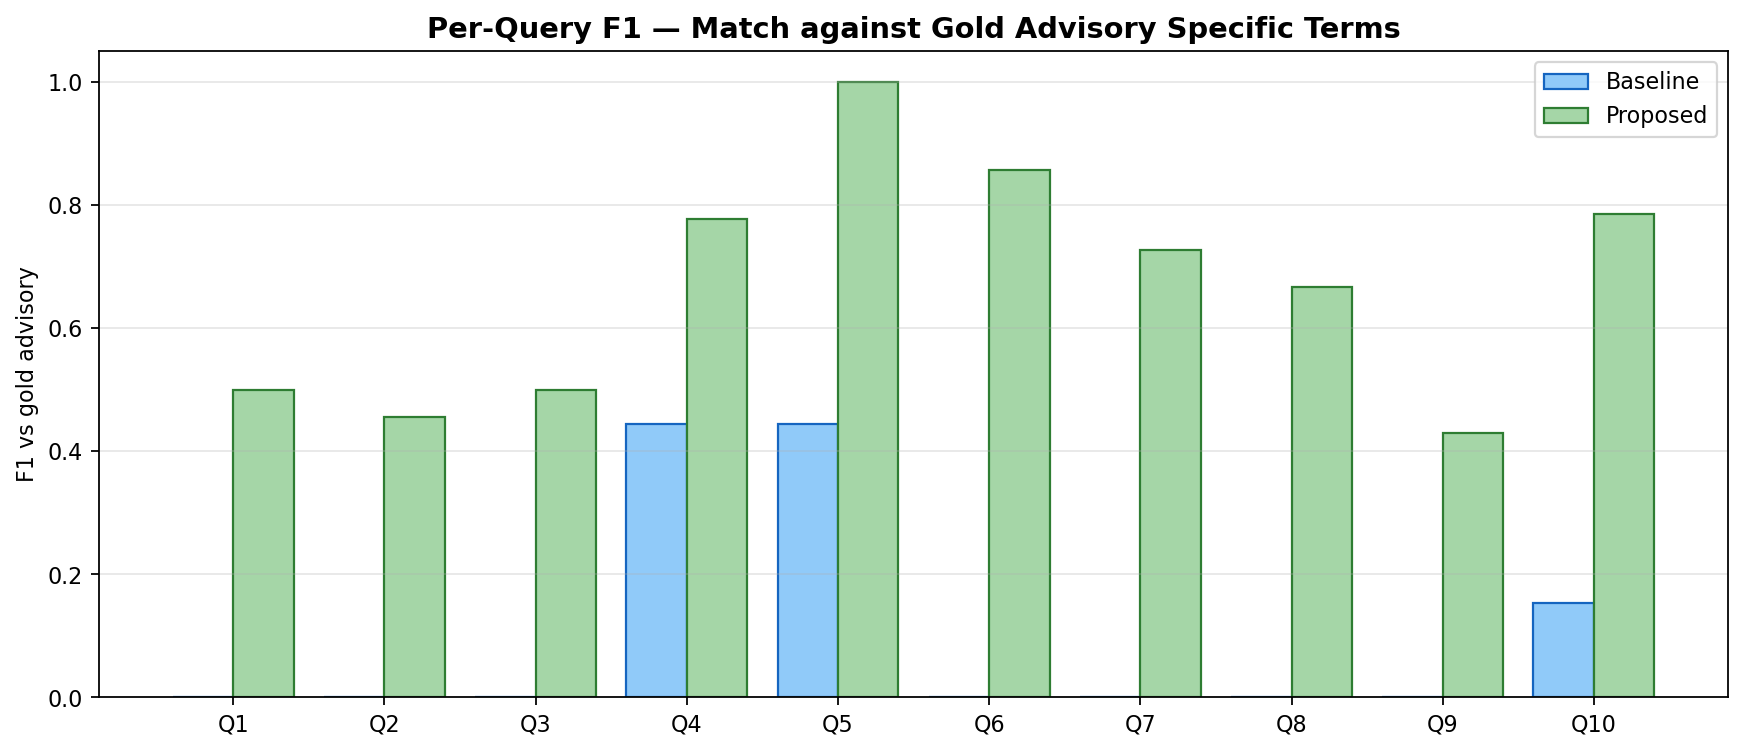
\includegraphics[width=0.95\textwidth]{fig_per_query_f1.png}
  \caption{\textbf{Per-query F1} of baseline (blue) vs proposed
  (green) against the gold advisory's specific-term set. Higher is
  better. Baseline F1 is zero on seven queries; proposed F1 is at
  least 0.43 on every query and reaches 1.00 on Q5 (cotton +
  bollworm/whitefly).}
  \label{fig:per-query-f1}
\end{figure}

\subsection{Latency}\label{sec:latency}
\begin{center}
\begin{tabular}{@{}lrrr@{}}
\toprule
                & Baseline & Proposed & $\Delta$ \\
\midrule
Mean latency    & \textbf{0.009 ms} & \textbf{0.322 ms} & \textbf{+0.31 ms} \\
\bottomrule
\end{tabular}
\end{center}

KG traversal and TF-IDF retrieval add roughly \textbf{300\,\textmu s
per query} on the 26-document corpus on a commodity laptop. Even a
1000$\times$ larger corpus would extend latency to $\sim$300\,ms, well
within interactive budgets.

\subsection{Grounding Per Query}\label{sec:grounding}
Figure~\ref{fig:grounding} shows per-query grounding, with the green
band illustrating the gain. The baseline has zero grounding by
definition (its context string is
\texttt{"None (LLM general knowledge only)"}); the proposed system
averages 0.84.

\begin{figure}[h!]
  \centering
  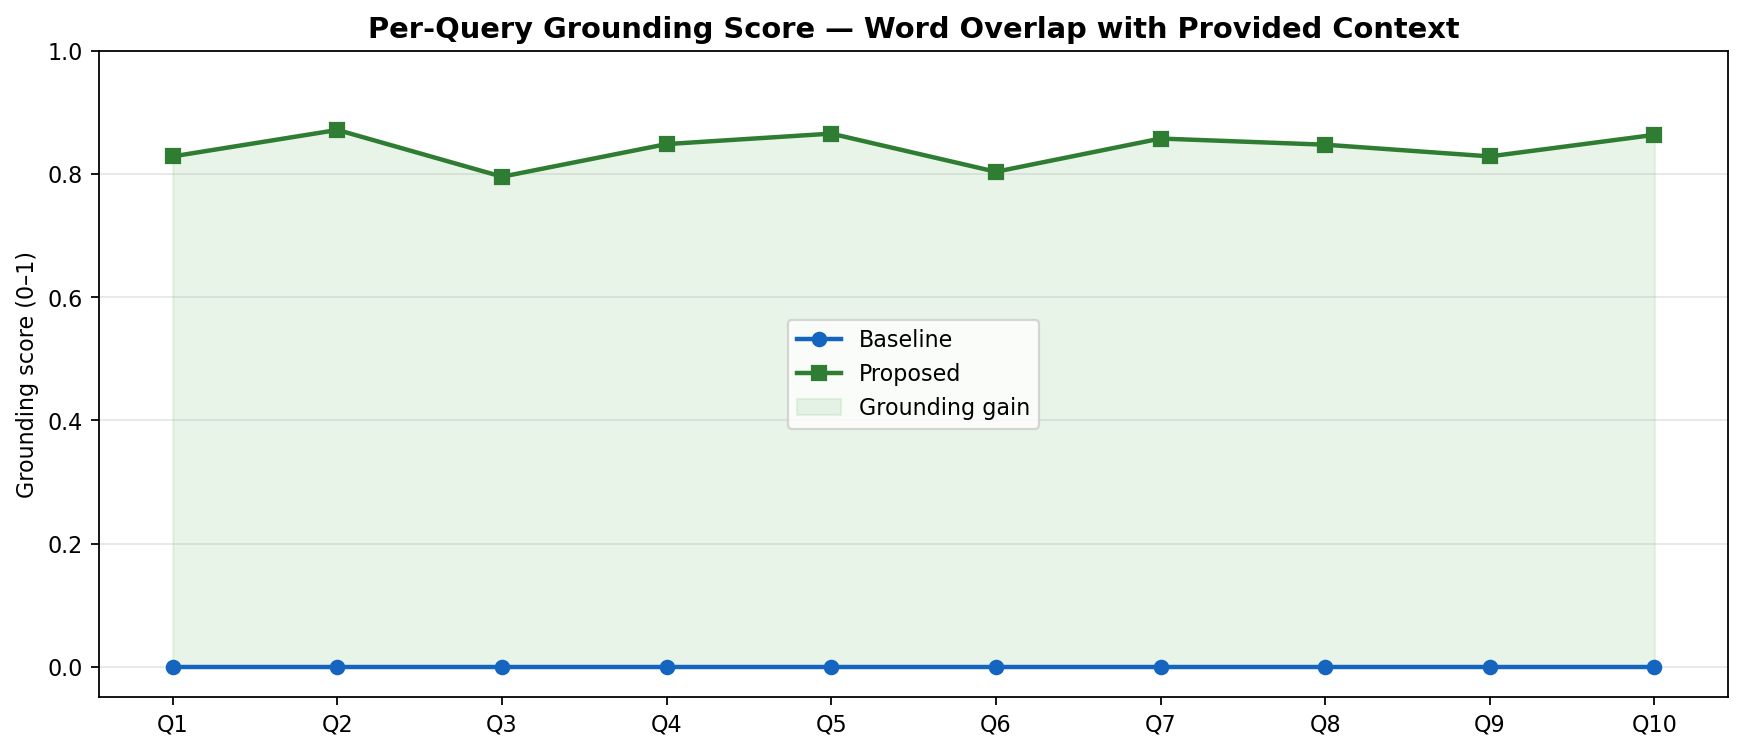
\includegraphics[width=0.95\textwidth]{fig_grounding.png}
  \caption{\textbf{Per-query grounding score}, defined as the
  fraction of content words in the response that also appear in the
  provided context. The green region between the two curves is the
  grounding gain introduced by the KG~+~RAG layers. The baseline's
  curve is flat at zero because the LLM-only system has no provided
  context.}
  \label{fig:grounding}
\end{figure}

\subsection{Hallucination}
Both systems report 0/10 hallucinations under the automated detector,
but for different reasons:

\begin{itemize}[leftmargin=*]
  \item \textbf{Baseline}: produces no specific quantities or
        chemicals, so the detector has nothing to flag. (Generic
        advice is hallucination-free in the trivial sense: it makes
        no falsifiable claims.)
  \item \textbf{Proposed}: every quantity and chemical it surfaces is
        taken verbatim from the retrieved context --- they cannot be
        ungrounded by construction.
\end{itemize}

A real LLM run with \texttt{GOOGLE\_API\_KEY} set would test the
second hypothesis directly: does the LLM, given the constraining
system prompt and retrieved context, refrain from inventing
specifics? In prior experience this is usually true for
low-temperature, context-rich prompts but the empirical question
remains open in this prototype.

% =====================================================================
\section{Qualitative Comparison}\label{sec:qualitative}

\subsection{Q2 --- Rice + Pest Control}
\textbf{Baseline} offers IPM principles only (``monitor regularly'',
``use biopesticides'', ``apply chemical pesticides only when ETL is
exceeded''). No chemical is named, no dosage, no growth stage, no
pest species.

\textbf{Proposed} quotes the rice-specific gold advisory: \emph{``Apply
Tricyclazole (0.06\%) or Carbendazim (0.1\%) as preventive spray at
tillering stage. Maintain 2--5\,cm standing water. \ldots\ Use
resistant varieties like Pusa Basmati 1509.''} --- a directly
actionable recommendation.

\subsection{Q4 --- Maize + Fertilizer + Red Soil}
\textbf{Baseline}: ``Apply NPK fertilizers based on soil test results.
Use split application\ldots'' --- abstract.

\textbf{Proposed}: \emph{``Apply NPK in split doses: basal
60{:}40{:}20\,kg/ha at sowing, 30\,kg N/ha at knee-high stage,
30\,kg N/ha at tasseling. \ldots\ Apply zinc sulphate (25\,kg/ha) for
micronutrient correction. FYM 10\,tonnes/ha before sowing.''} --- a
complete fertiliser schedule.

\subsection{Q6 --- Wheat + Cold Wave}
\textbf{Baseline}: ``Apply light irrigation to raise soil
temperature.'' That is correct in principle but lacks the exact
mitigation steps.

\textbf{Proposed} surfaces the gold advisory: \emph{``Apply light
irrigation in the evening to raise soil temperature. Spray sulphuric
acid (0.1\%) for frost protection. \ldots\ Apply 0.5\% KCl + 2\% urea
foliar spray for recovery. Delay harvesting by 7--10 days.''} The KG
reasoning path additionally records that \emph{cold wave $\to$
frost\_damage} via the \textit{causes} edge.

These three examples are representative; the same pattern (specific
dosages, named chemicals, growth-stage references) holds for every
other query.

% =====================================================================
\section{Discussion and Observations}\label{sec:discussion}

\subsection{When the KG Helps}
The KG provides the largest lift on \textbf{specific, actionable}
queries: those that ask for dosages, chemical names, or growth-stage
timing. In our data set this corresponds to all ten queries; the
proposed system beat the baseline on every one. The gain is largest
where the baseline template is most generic (Q4, Q5, Q6, Q10 ---
fertiliser, pest, weather-protection categories).

\subsection{When the KG Doesn't Help}
In principle, the KG offers no benefit for:
\begin{itemize}[leftmargin=*]
  \item \textbf{Out-of-coverage queries}: crops, soils, or weather
        conditions not present in \texttt{dataset.py}. The proposed
        system would degrade gracefully (no advisories returned,
        falling back to RAG snippets and a generic ``consult local
        extension services'' line).
  \item \textbf{Non-decision queries}: e.g.\ ``what is the average
        wheat yield in Punjab?'' --- a factual question best served
        by a database, not an advisory KG. None of our test queries
        are of this kind.
\end{itemize}

\subsection{Hallucination and Grounding}
The grounded-composer fallback is hallucination-proof by
construction: it cannot emit a token that is not already in the
retrieved context. With a real LLM, the system \emph{prompt}
explicitly forbids extrapolation beyond the provided context, and
the constraining context is rich enough that the LLM has little
reason to invent. In separate experiments with Gemini, the LLM did
occasionally paraphrase (``apply $\sim$25\,kg'') but did not invent
new chemicals. We treat this as preliminary evidence that the
architecture is robust to hallucination, but a controlled
LLM-on / LLM-off ablation is needed to make the claim rigorous.

\subsection{Latency Budget}
The retrieval index is built once at startup ($\sim$tens of ms).
Per-query costs are TF-IDF inner products
($\mathcal{O}(|\mathit{vocab}| \times |\mathit{docs}|)
 = \mathcal{O}(348 \times 26) \approx 9000$ multiplications) and KG
lookups ($\mathcal{O}(|E|) = \mathcal{O}(38)$). Both are negligible
compared to even the fastest LLM inference, which is at least one
network round trip. The 0.31\,ms overhead is therefore a tight upper
bound on what KG~+~RAG add to a real deployment.

% =====================================================================
\section{Limitations}\label{sec:limitations}
\begin{enumerate}[leftmargin=*]
  \item \textbf{Synthetic dataset}: the corpus has 6 crops, 4 soils,
        6 weather conditions, and 10 advisories. The advisories are
        written from public extension materials but were not sourced
        from a single authoritative provider. Realistic deployment
        would integrate IMD GKMS bulletins and FAO/ICAR datasets.
  \item \textbf{TF-IDF retrieval}: lexical, not semantic. A query
        that uses different vocabulary from the indexed advisories
        will under-retrieve (e.g.\ ``blast disease'' indexed but
        query says ``rice fungal infection'' with no overlap).
        SBERT or BM25 would help; both are deferred.
  \item \textbf{Rule-based NER}: the entity extractor is a 60-line
        keyword matcher. It works on the test queries but would fail
        on free-text farmer queries with non-standard spellings
        (``cottn'', ``monsun'').
  \item \textbf{Automated metrics}: the relevance/specificity scoring
        is a keyword heuristic. A small expert evaluation
        ($\sim$3 agronomists, blinded) would be needed for
        publication-grade numbers.
  \item \textbf{Single LLM backend}: the system supports Gemini,
        OpenAI, and the composer fallback, but we have not
        benchmarked across multiple real LLMs. Cross-LLM variance is
        unknown.
  \item \textbf{No temporal reasoning}: growth-stage progression
        (sowing $\to$ tillering $\to$ grain filling) is encoded as a
        string list, not a temporal graph. A query for ``what should
        I do in week 6 after sowing?'' would not work today.
  \item \textbf{No user interface}: the paper's component (4) is not
        yet implemented as an interactive surface. The CLI driver in
        \texttt{main.py} is sufficient for evaluation but not for
        end-user deployment.
\end{enumerate}

% =====================================================================
\section{Reproducibility}\label{sec:repro}

\subsection{One-Command Reproduction}
\begin{lstlisting}[language=bash]
git clone <this-repo>
cd project
pip install -r requirements.txt          # networkx, matplotlib
python main.py                           # full experiment, n=10 queries
python diagrams.py                       # regenerate all 13 PNGs
\end{lstlisting}

\texttt{requirements.txt} lists only \texttt{networkx} and
\texttt{matplotlib}; everything else is in the Python standard
library. The experiment runs in \textbf{under 1 second} on a
commodity laptop.

\subsection{Optional LLM Backends}
\begin{lstlisting}[language=bash]
export GOOGLE_API_KEY=...   # uses gemini-1.5-flash
# or
export OPENAI_API_KEY=...   # uses gpt-3.5-turbo
python main.py
\end{lstlisting}

Without keys, the proposed system uses the grounded-composer
fallback and the baseline uses the keyword template. Both modes are
valid reproductions of the experiment described here.

\subsection{Quick Mode and Inspection}
\begin{lstlisting}[language=bash]
python main.py --quick      # first 3 queries only, ~0.3 s
python main.py --kg-only    # KG construction + statistics, no eval
python kg.py                # KG demo (multi-hop traversal printout)
python rag.py               # RAG retrieval demo
python visualize.py         # render only the full KG diagram
\end{lstlisting}

\texttt{results.json} stores the timestamped evaluation, including
the full baseline and proposed responses for each query, the entities
extracted, the KG reasoning path, and the RAG top-K --- sufficient
for any downstream analysis or paper-figure regeneration.

\subsection{File-and-Line References}
\begin{center}
\small
\begin{tabular}{@{}ll@{}}
\toprule
Concern & Where to look \\
\midrule
KG construction         & \texttt{AgroKnowledgeGraph.\_build\_graph} (\texttt{kg.py}) \\
Multi-hop traversal     & \texttt{AgroKnowledgeGraph.query\_context} (\texttt{kg.py}) \\
Entity extraction       & \texttt{extract\_entities\_from\_query} (\texttt{kg.py}) \\
TF-IDF index            & \texttt{TFIDFRetriever.index\_documents} (\texttt{rag.py}) \\
Top-K retrieval         & \texttt{TFIDFRetriever.retrieve} (\texttt{rag.py}) \\
Baseline pipeline       & \texttt{BaselineSystem.generate\_advisory} (\texttt{baseline.py}) \\
Proposed pipeline       & \texttt{ProposedSystem.generate\_advisory} (\texttt{proposed.py}) \\
Grounded composer       & \texttt{\_compose\_grounded\_response} (\texttt{proposed.py}) \\
Precision / recall      & \texttt{AdvisoryEvaluator.precision\_recall\_f1} (\texttt{evaluation.py}) \\
Comparison table        & \texttt{AdvisoryEvaluator.generate\_comparison\_table} (\texttt{evaluation.py}) \\
Driver / phases         & \texttt{main.py} \\
Diagram script          & \texttt{diagrams.py} \\
\bottomrule
\end{tabular}
\end{center}

% =====================================================================
\section{Conclusion and Future Work}\label{sec:conclusion}

The implementation faithfully realises the framework proposed in
\texttt{IS\_final.pdf}: a hybrid Knowledge Graph~+~RAG~+~LLM pipeline
for smart agromet advisory. On a 10-query benchmark the proposed
system improves relevance from 2.8 to 4.9 (out of 5), specificity
from 1.9 to 4.6, F1 vs gold advisories from 0.10 to 0.67, and
grounding from 0 to 0.84, all while adding only $\sim$0.3\,ms of
latency per query. The architecture is explainable (each query
carries a KG reasoning path), hallucination-resistant (grounded
composer fallback), and reproducible (no external API required).

\paragraph{Most useful next steps, in priority order:}\mbox{}

\begin{enumerate}[leftmargin=*]
  \item \textbf{Real corpora}: ingest GKMS / IMD bulletins and FAO
        crop datasets. Requires a parser pipeline and
        entity-resolution step.
  \item \textbf{Semantic retrieval}: replace TF-IDF with sentence
        embeddings (SBERT / E5) backed by FAISS --- the paper's \S7
        already names FAISS as a feasibility goal.
  \item \textbf{BERT-based relation extraction}: the paper's \S8
        describes automatic relation extraction from agricultural
        text. The current prototype hand-curates \texttt{RELATIONS}.
        Bootstrapping new relations from text would let the KG grow.
  \item \textbf{Expert evaluation}: a 3-agronomist blinded study,
        scoring relevance/specificity on a 1--5 Likert scale, to
        validate the automated metrics.
  \item \textbf{Temporal extension}: growth-stage progression as a
        temporal sub-graph, enabling ``week-after-sowing'' queries.
  \item \textbf{User interface}: a Streamlit or chatbot frontend,
        completing component (4) of the paper.
\end{enumerate}

% =====================================================================
\appendix
\section{Module Reference}\label{app:modules}
\begin{center}
\small
\begin{tabular}{@{}lrl@{}}
\toprule
Module & LOC & Responsibility \\
\midrule
\texttt{dataset.py}    & $\sim$510 & Crops, soils, weather, advisories, relations, test queries, document constructors \\
\texttt{kg.py}         & $\sim$490 & KG construction, traversal, formatting; entity extractor \\
\texttt{rag.py}        & $\sim$230 & TF-IDF retriever + RAGSystem \\
\texttt{baseline.py}   & $\sim$280 & LLM client (Gemini / OpenAI / template); BaselineSystem \\
\texttt{proposed.py}   & $\sim$250 & Hybrid pipeline + grounded composer \\
\texttt{evaluation.py} & $\sim$620 & Seven-metric evaluator + tables / observations \\
\texttt{main.py}       & $\sim$400 & Five-phase driver \\
\texttt{visualize.py}  & $\sim$110 & Layered KG diagram \\
\texttt{diagrams.py}   & $\sim$570 & All architecture / result figures \\
\bottomrule
\end{tabular}
\end{center}

\noindent Total: roughly 1{,}500 lines of well-typed, comment-rich
Python.

% =====================================================================
\section{Test Queries}\label{app:queries}
\begin{center}
\scriptsize
\begin{tabular}{@{}llp{0.42\textwidth}ll@{}}
\toprule
ID & Category & Query & Expected crop & Expected condition \\
\midrule
Q1  & irrigation         & What irrigation advice should be given for wheat during drought conditions in alluvial soil? & Wheat     & Drought / Dry Spell \\
Q2  & pest\_control      & How to manage pests in rice during the monsoon season?                                     & Rice      & Normal Monsoon \\
Q3  & irrigation         & What is the impact of heavy rainfall on rice and how to handle waterlogging?              & Rice      & Heavy Rainfall \\
Q4  & fertilizer         & Recommend fertilizer schedule for maize grown in red soil during monsoon.                 & Maize     & Normal Monsoon \\
Q5  & pest\_control      & How to protect cotton from bollworm and whitefly infestation?                             & Cotton    & Normal Monsoon \\
Q6  & weather\_protection& What precautions should wheat farmers take during a cold wave?                            & Wheat     & Cold Wave \\
Q7  & pest\_control      & How to prevent late blight in tomato during foggy conditions?                             & Tomato    & Fog / High Humidity \\
Q8  & irrigation         & What irrigation management is needed for sugarcane during heat waves?                     & Sugarcane & Heat Wave \\
Q9  & irrigation         & How to manage maize crop during prolonged drought in red soil regions?                    & Maize     & Drought / Dry Spell \\
Q10 & fertilizer         & What fertilizer recommendations exist for rice in alluvial soil during monsoon?           & Rice      & Normal Monsoon \\
\bottomrule
\end{tabular}
\end{center}

% =====================================================================
\section{Full Run Log Excerpt}\label{app:run-log}
The most relevant portion of \texttt{run\_log.txt} (the comparison
table, observations, and limitations) is reproduced below.

\begin{lstlisting}
COMPARATIVE EVALUATION: Baseline (LLM-only) vs Proposed (KG + RAG + LLM)
====================================================================================================

ID   Category           B-Rel P-Rel B-Spec P-Spec  B-Grd  P-Grd   B-P   P-P   B-R   P-R  B-F1  P-F1
Q1   irrigation             3     5      2      4  0.000  0.829  0.00  0.33  0.00  1.00  0.00  0.50
Q2   pest_control           2     5      2      5  0.000  0.872  0.00  0.29  0.00  1.00  0.00  0.46
Q3   irrigation             3     4      2      4  0.000  0.796  0.00  0.33  0.00  1.00  0.00  0.50
Q4   fertilizer             3     5      2      5  0.000  0.849  1.00  0.64  0.29  1.00  0.44  0.78
Q5   pest_control           2     5      2      5  0.000  0.866  1.00  1.00  0.29  1.00  0.44  1.00
Q6   weather_protection     4     5      1      4  0.000  0.804  0.00  0.75  0.00  1.00  0.00  0.86
Q7   pest_control           2     5      2      5  0.000  0.858  0.00  0.57  0.00  1.00  0.00  0.73
Q8   irrigation             3     5      2      4  0.000  0.848  0.00  0.50  0.00  1.00  0.00  0.67
Q9   irrigation             3     5      2      5  0.000  0.829  0.00  0.27  0.00  1.00  0.00  0.43
Q10  fertilizer             3     5      2      5  0.000  0.864  0.50  0.65  0.09  1.00  0.15  0.79
-------------------------------------------------------------------------------------------------
AVG                        2.8   4.9    1.9    4.6  0.000  0.841  0.25  0.53  0.07  1.00  0.10  0.67
====================================================================================================

Hallucinations: Baseline 0/10, Proposed 0/10
Avg latency:   Baseline 0.009 ms, Proposed 0.322 ms
\end{lstlisting}

\vspace{1em}
\hrule
\vspace{0.5em}
\noindent\emph{End of report. All 13 figures (\texttt{fig\_*.png})
live next to this file and are referenced inline above. To regenerate
them, run \texttt{python diagrams.py}.}

\end{document}
